
%   Hamzeh Khanpour
%   DIS 2026 talk
%   Perspectives for HET physics studies at a muon-hadron collider at CERN


\documentclass[aspectratio=1610,english]{beamer}

\usepackage{babel}
\usepackage[T1]{fontenc}
\usepackage[utf8]{inputenc}
\usepackage{lmodern}
\usepackage{amsmath,amssymb,bm}
\usepackage{booktabs}
\usepackage{graphicx}
\usepackage{array}
\usepackage{ragged2e}
\usepackage{etoolbox}


\usepackage{tikz}
\usepackage{comment}

\usepackage{tikz-feynman}
\tikzfeynmanset{compat=1.1.0}


\usetikzlibrary{calc,positioning,arrows.meta,decorations.pathmorphing,patterns,shapes.geometric}

\usepackage{hyperref}

\usepackage[table]{xcolor}

\makeatletter
\patchcmd{\itemize}{\raggedright}{\justifying}{}{}
\patchcmd{\beamer@enum@}{\raggedright}{\justifying}{}{}
\patchcmd{\@@description}{\raggedright}{\justifying}{}{}
\makeatother

\mode<beamer>{
    \definecolor{links}{HTML}{2A1B81}
    \hypersetup{pdfpagemode=FullScreen,colorlinks,linkcolor=,urlcolor=links}
    \usetheme[parttitle=rightfooter]{AGH}
}

\graphicspath{{./}{/mnt/data/}}

\definecolor{LHRed}{RGB}{170,20,30}
\definecolor{LHBlue}{RGB}{25,60,180}
\definecolor{LHGreen}{RGB}{0,120,60}
\definecolor{LHOrange}{RGB}{210,110,20}
\definecolor{LHPurple}{RGB}{110,60,160}



\newcommand{\LHCmu}{LH$\mu$C}
\newcommand{\placeholdergraphic}[2]{%
\begin{center}
\fbox{\parbox[c][#2][c]{0.86\textwidth}{\centering\vspace{1ex}\textbf{Placeholder for later screenshot}\\[0.6ex]\small #1\vspace{1ex}}}
\end{center}}



\newcommand{\takehome}[1]{%
\begin{alertblock}{Take-home message}
\small #1
\end{alertblock}}



\title[DIS 2026 report for HELP4CERN]{\justifying DIS 2026 report: HELP4CERN contributions and WG-summary visibility}
\author[Hamzeh Khanpour]{Hamzeh Khanpour\\
{\scriptsize \href{}{AGH University of Krakow}}}


\institute[AGH]{\color{magenta}\textbf{(on behalf of HELP4CERN Study Group)}}


\date{{\setlength{\fboxsep}{4pt}\colorbox{cyan!15}{\strut HELP4CERN collaboration report - DIS 2026, Bologna}}}
 
 

% \textbf{Contact:} \texttt{help-4-cern@cern.ch}





% --------------------------------------------------------------------------
% Local helper boxes for the DIS 2026 report slides
% --------------------------------------------------------------------------
\newcommand{\reportlogonorth}{%
\begin{tikzpicture}[remember picture,overlay]
\node[anchor=north east, xshift=-0.10cm, yshift=-0.35cm]
at (current page.north east)
{
\includegraphics[width=1.45cm]{HELP4CERN.jpg}};
\end{tikzpicture}}

\newcommand{\indicolink}[2]{\href{#1}{\scriptsize #2}}

\newcommand{\wgscreenshot}[5]{%
\begin{frame}{#1}
\begin{columns}[T,totalwidth=\textwidth]
\begin{column}{0.70\textwidth}
\centering
\includegraphics[width=\linewidth,height=0.74\textheight,keepaspectratio]{#2}
\end{column}
\begin{column}{0.28\textwidth}
\begin{block}{Why it matters}
\scriptsize
\begin{itemize}
\justifying
#3
\end{itemize}
\end{block}
\vspace{0.3em}
{\scriptsize\color{gray}#4}
\end{column}
\end{columns}
\reportlogonorth
\end{frame}}

\begin{document}
 
% --------------------------------------------------------------------------
% Slide 1
% --------------------------------------------------------------------------
\begin{frame}
\begin{tikzpicture}[remember picture,overlay]
\node[anchor=north east, xshift=-0.60cm, yshift=-1.50cm]
at (current page.north east)
{
\includegraphics[width=2.5cm]{HELP4CERN.jpg}};
\end{tikzpicture}
\titlepage
\end{frame}

% --------------------------------------------------------------------------
% Slide 2
% --------------------------------------------------------------------------
\begin{frame}{Outline}
\tableofcontents
\begin{tikzpicture}[remember picture,overlay]
\node[anchor=north east, xshift=-0.60cm, yshift=-1.50cm]
at (current page.north east)
{
\includegraphics[width=2.5cm]{HELP4CERN.jpg}};
\end{tikzpicture}
\end{frame}



\section{DIS 2026 context}

% --------------------------------------------------------------------------
% Slide 3
% --------------------------------------------------------------------------
\begin{frame}{DIS 2026 as a visibility point for HELP4CERN}
\begin{columns}[T]%[T,totalwidth=\textwidth]
\begin{column}{0.58\textwidth}
\begin{block}{Main message from DIS 2026}
\small
\begin{itemize}
\justifying
\item The HELP4CERN programme was visible across several DIS 2026 working groups: machine concept, detector/staging, small-$x$ QCD, and HET physics.
\item The proposed LH$\mu$C was discussed as a possible high-energy lepton--hadron extension at CERN, not simply as an energy upgrade of the LHeC.
\item The WG-summary slides gave useful external feedback on where the community sees the strongest physics and strategy questions.
\end{itemize}
\end{block}

%\begin{alertblock}{Collaboration-level take-away}
%\scriptsize
%\justifying
%DIS 2026 helped connect the LH$\mu$C/LHeC physics case to concrete questions for the HELP4CERN white paper: physics benchmarks, detector realism, accelerator staging, and European-strategy positioning.
%\end{alertblock}

\end{column}

\begin{column}{0.39\textwidth}
\begin{exampleblock}{Four DIS contributions reviewed}
\scriptsize
\begin{itemize}
\justifying
\item K. Piotrzkowski: LH$\mu$C concept and programme.
\item L. Forthomme: LHeC/FCC-eh detector and staging.
\item P. Kotko: high-energy QCD and small-$x$ reach.
\item H. Khanpour: HET physics at a muon--hadron collider.
\end{itemize}
\end{exampleblock}

\begin{block}{WG-summary visibility}
\scriptsize
\begin{itemize}
\justifying
\item WG2: small-$x$ and $Q^2$--$x$ plane.
\item WG3: HET physics prospects at LH$\mu$C.
\item WG6: machine, detector and strategy outlook.
\end{itemize}
\end{block}

\end{column}
\end{columns}
\reportlogonorth
\end{frame}

% --------------------------------------------------------------------------
% Slide 4
% --------------------------------------------------------------------------
\begin{frame}{Report structure: from talks to next steps}
\begin{columns}[T]%[T,totalwidth=\textwidth]
\begin{column}{0.99\textwidth}
\begin{block}{What this report summarizes}
\small
\begin{itemize}
\justifying
\item Four HELP4CERN-related DIS 2026 presentations.
\item How these studies appeared in WG-summary material.
\item Physics and technical feedback to sharpen for the white paper.
\item ICHEP 2026 as the next opportunity for a coherent presentation.
\end{itemize}
\end{block}
\end{column}

\end{columns}

\vspace{0.5em}
\begin{center}
{\scriptsize DIS 2026 contribution pages: \href{https://agenda.infn.it/event/47074/contributions/289190/}{289190},
\href{https://agenda.infn.it/event/47074/contributions/289187/}{289187},
\href{https://agenda.infn.it/event/47074/contributions/289240/}{289240},
\href{https://agenda.infn.it/event/47074/contributions/289107/}{289107}.}
\end{center}
\reportlogonorth
\end{frame}

\section{Four DIS 2026 HELP4CERN contributions}

% --------------------------------------------------------------------------
% Slide 5
% --------------------------------------------------------------------------
\begin{frame}{DIS 2026 contribution: Krzysztof Piotrzkowski}
\begin{columns}[T]%[T,totalwidth=\textwidth]
\begin{column}{0.60\textwidth}
\begin{block}{Talk}
\small
\textbf{LH$\mu$C: A high energy, high luminosity muon-hadron collider at CERN}\\[0.25em]
{\scriptsize K. Piotrzkowski, WG6 Current Upgrades and Future Experiments, 5 May 2026.}
\end{block}

\begin{block}{Physics and concept message}
\scriptsize
\begin{itemize}
\justifying
\item Presented the LH$\mu$C concept based on reusing elements of the LHeC ERL infrastructure.
\item Baseline example: a $500~\mathrm{GeV}$ $\mu^+$ beam colliding with the $7~\mathrm{TeV}$ LHC proton beam, giving $\sqrt{s}\simeq3.74~\mathrm{TeV}$.
\item Discussed the path from ultra-cold $\mu^+$ production to booster/ring concepts and first machine--detector-interface issues.
\item Framed the scientific programme from QCD and DIS to HET and representative BSM studies.
\end{itemize}
\end{block}
\end{column}

\begin{column}{0.40\textwidth}
\begin{exampleblock}{HELP4CERN relevance}
\scriptsize
\begin{itemize}
\justifying
\item Provides the common accelerator and staging narrative for the white paper.
\item Makes the physics--machine connection explicit: luminosity, energy, detector protection and feasibility.
\item Connects LH$\mu$C to LHeC, muon-collider and FCC discussions.
\end{itemize}
\end{exampleblock}


{\scriptsize \href{https://agenda.infn.it/event/47074/contributions/289190/}{DIS 2026 Indico contribution 289190}}
\end{column}
\end{columns}
\reportlogonorth
\end{frame}

% --------------------------------------------------------------------------
% Slide 6
% --------------------------------------------------------------------------
\begin{frame}{DIS 2026 contribution: Laurent Forthomme}
\begin{columns}[T]%[T,totalwidth=\textwidth]
\begin{column}{0.60\textwidth}
\begin{block}{Talk}
\small
\textbf{A detector for top energy DIS}\\[0.25em]
{\scriptsize L. Forthomme, WG6 Current Upgrades and Future Experiments, 5 May 2026.}
\end{block}

\begin{block}{Detector and staging message}
\scriptsize
\begin{itemize}
\justifying
\item Reviewed the status of detector concepts for top-energy DIS at the LHeC and extension toward FCC-eh.
\item Used the LHeC idea of electron--proton/nucleus collisions at CERN with an ERL electron beam as the near-term reference.
\item Discussed staged LHeC operation as a bridge from HL-LHC toward a possible later flagship collider.
\item Highlighted synergies with ALICE~3, ePIC and future $e^+e^-$ detector concepts.
\end{itemize}
\end{block}
\end{column}

\begin{column}{0.40\textwidth}
\begin{exampleblock}{HELP4CERN relevance}
\scriptsize
\begin{itemize}
\justifying
\item Gives the detector realism needed for a credible lepton--hadron programme.
\item Provides a reference geometry for later LH$\mu$C detector and MDI discussions.
\item Helps separate near-term LHeC questions from more speculative LH$\mu$C extensions.
\end{itemize}
\end{exampleblock}


{\scriptsize \href{https://agenda.infn.it/event/47074/contributions/289187/}{DIS 2026 Indico contribution 289187}}
\end{column}
\end{columns}
\reportlogonorth
\end{frame}

% --------------------------------------------------------------------------
% Slide 7
% --------------------------------------------------------------------------
\begin{frame}{DIS 2026 contribution: Piotr Kotko}
\begin{columns}[T]%[T,totalwidth=\textwidth]
\begin{column}{0.60\textwidth}
\begin{block}{Talk}
\small
\textbf{Exploring the frontier of high energy QCD with the LH$\mu$C}\\[0.25em]
{\scriptsize P. Kotko, WG2 Small-$x$, Diffraction and Vector Mesons, 6 May 2026.}
\end{block}

\begin{block}{QCD message}
\scriptsize
\begin{itemize}
\justifying
\item Presented LH$\mu$C as a high-energy DIS facility with access to extremely small Bjorken-$x$.
\item Emphasized potential reach down to $x\sim10^{-7}$ at perturbative virtualities around $Q^2\simeq1~\mathrm{GeV}^2$.
\item Motivated studies of gluon saturation, nonlinear QCD evolution and nuclear effects.
\item Highlighted the complementary large-$Q^2$, low-$x$ lever arm for PDF uncertainties and possible $\alpha_s$ extractions.
\end{itemize}
\end{block}
\end{column}

\begin{column}{0.40\textwidth}
\begin{exampleblock}{HELP4CERN relevance}
\scriptsize
\begin{itemize}
\justifying
\item Supplies one of the clearest visual arguments for the LH$\mu$C: the extended $Q^2$--$x$ plane.
\item Connects the proposal naturally to EIC, HERA, LHeC and FCC-eh comparisons.
\item Defines concrete QCD benchmarks for the white paper.
\end{itemize}
\end{exampleblock}


{\scriptsize \href{https://agenda.infn.it/event/47074/contributions/289240/}{DIS 2026 Indico contribution 289240}}
\end{column}
\end{columns}
\reportlogonorth
\end{frame}

% --------------------------------------------------------------------------
% Slide 8
% --------------------------------------------------------------------------
\begin{frame}{DIS 2026 contribution: Hamzeh Khanpour}
\begin{columns}[T]%[T,totalwidth=\textwidth]
\begin{column}{0.60\textwidth}
\begin{block}{Talk}
\small
\textbf{Perspectives for studies of the HET physics at the muon-hadron collider at CERN}\\[0.25em]
{\scriptsize H. Khanpour, WG3 Electroweak Physics, Top, Higgs and BSM, 7 May 2026.}
\end{block}

\begin{block}{HET message}
\scriptsize
\begin{itemize}
\justifying
\item Presented benchmark inclusive cross sections for Higgs and key top-quark processes at LH$\mu$C working points.
\item Highlighted opportunities for charged-current Higgs production and precision Higgs-coupling studies.
\item Discussed a broader electroweak/top programme, including high-$Q^2$ sensitivity and rare-top directions.
\item Included photon-induced processes and long-term muon--hadron options at FCC-hh energies.
\end{itemize}
\end{block}
\end{column}

\begin{column}{0.40\textwidth}
\begin{exampleblock}{HELP4CERN relevance}
\scriptsize
\begin{itemize}
\justifying
\item Establishes the HET pillar of the LH$\mu$C physics case.
\item Provides comparison points for HL-LHC, LHeC, FCC-ee and FCC-hh discussions.
\item Identifies where dedicated simulations and coupling-fit assumptions must be sharpened.
\end{itemize}
\end{exampleblock}


{\scriptsize \href{https://agenda.infn.it/event/47074/contributions/289107/}{DIS 2026 Indico contribution 289107}}
\end{column}
\end{columns}
\reportlogonorth
\end{frame}

\section{Visibility in DIS 2026 WG summaries}

% --------------------------------------------------------------------------
% Slide 9
% --------------------------------------------------------------------------

\begin{frame}{WG3 summary: LH$\mu$C HET physics highlighted}
	\begin{center}
		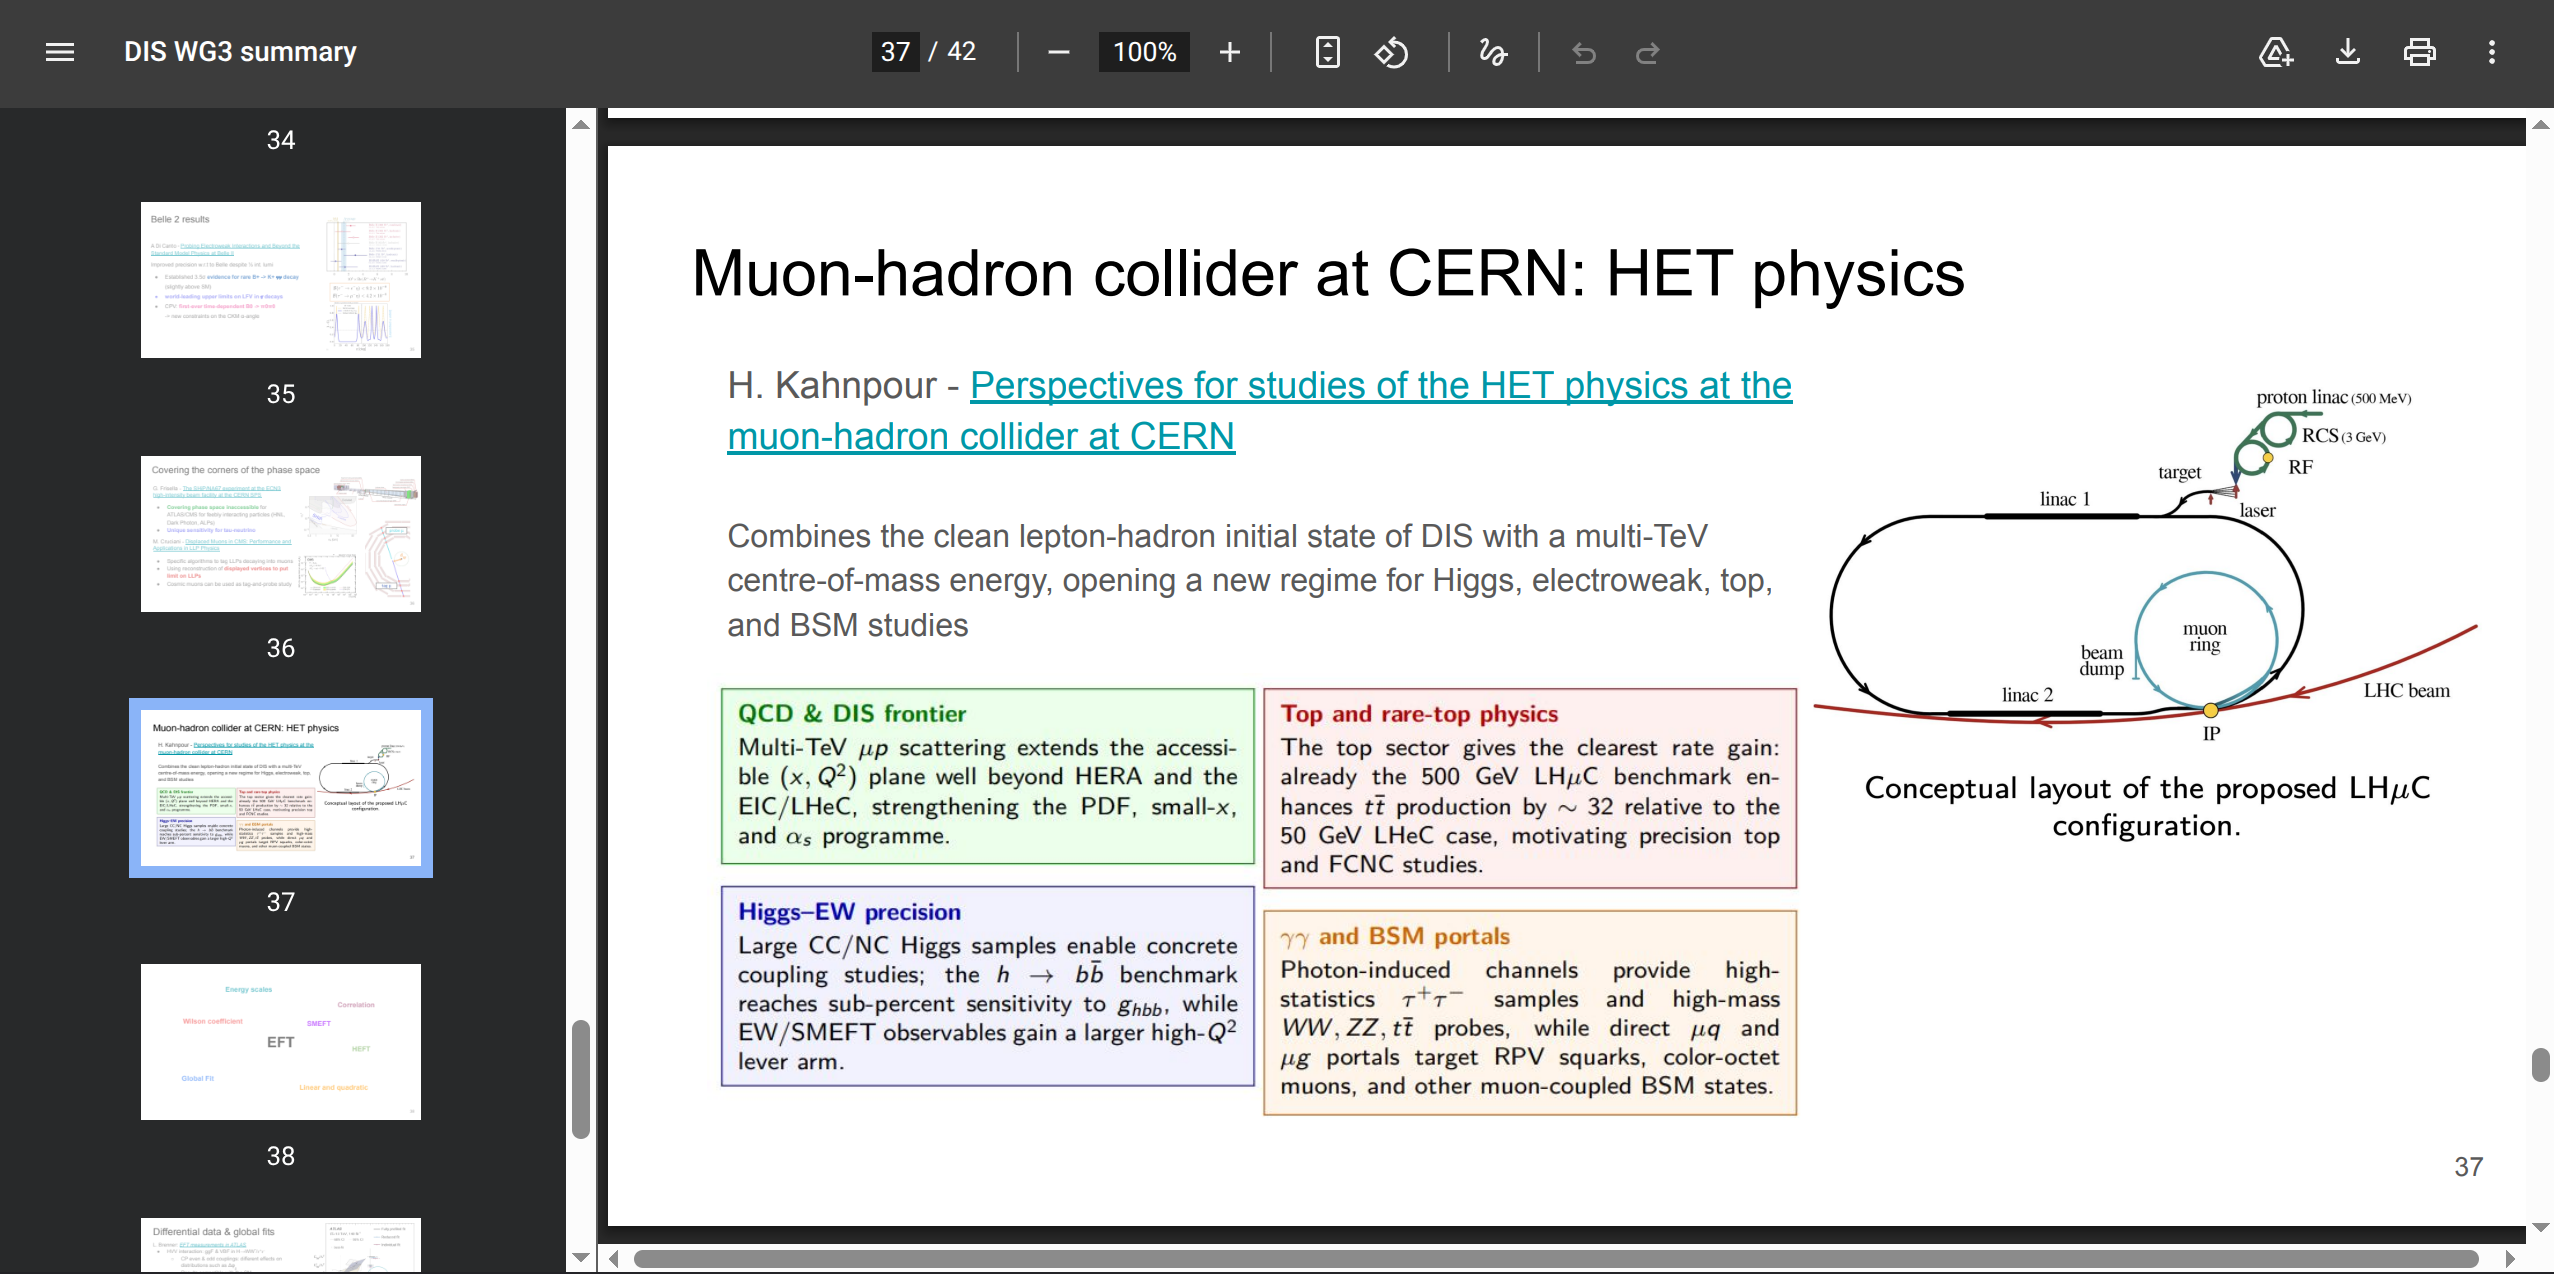
\includegraphics[width=0.85\paperwidth,height=0.85\paperheight,keepaspectratio]{Ha_1.png}
	\end{center}
	%------------------------------------------------
	% HELP4CERN logo overlay
	%------------------------------------------------
	\begin{tikzpicture}[remember picture,overlay]
		\node[anchor=north east, xshift=-0.55cm, yshift=-0.40cm]
		at (current page.north east)
		{
\includegraphics[width=1.5cm]{HELP4CERN.jpg}};
	\end{tikzpicture}
\end{frame}

% --------------------------------------------------------------------------
% Slide 10
% --------------------------------------------------------------------------


\begin{frame}{WG6 summary: LH$\mu$C concept and timeline}
	\begin{center}
		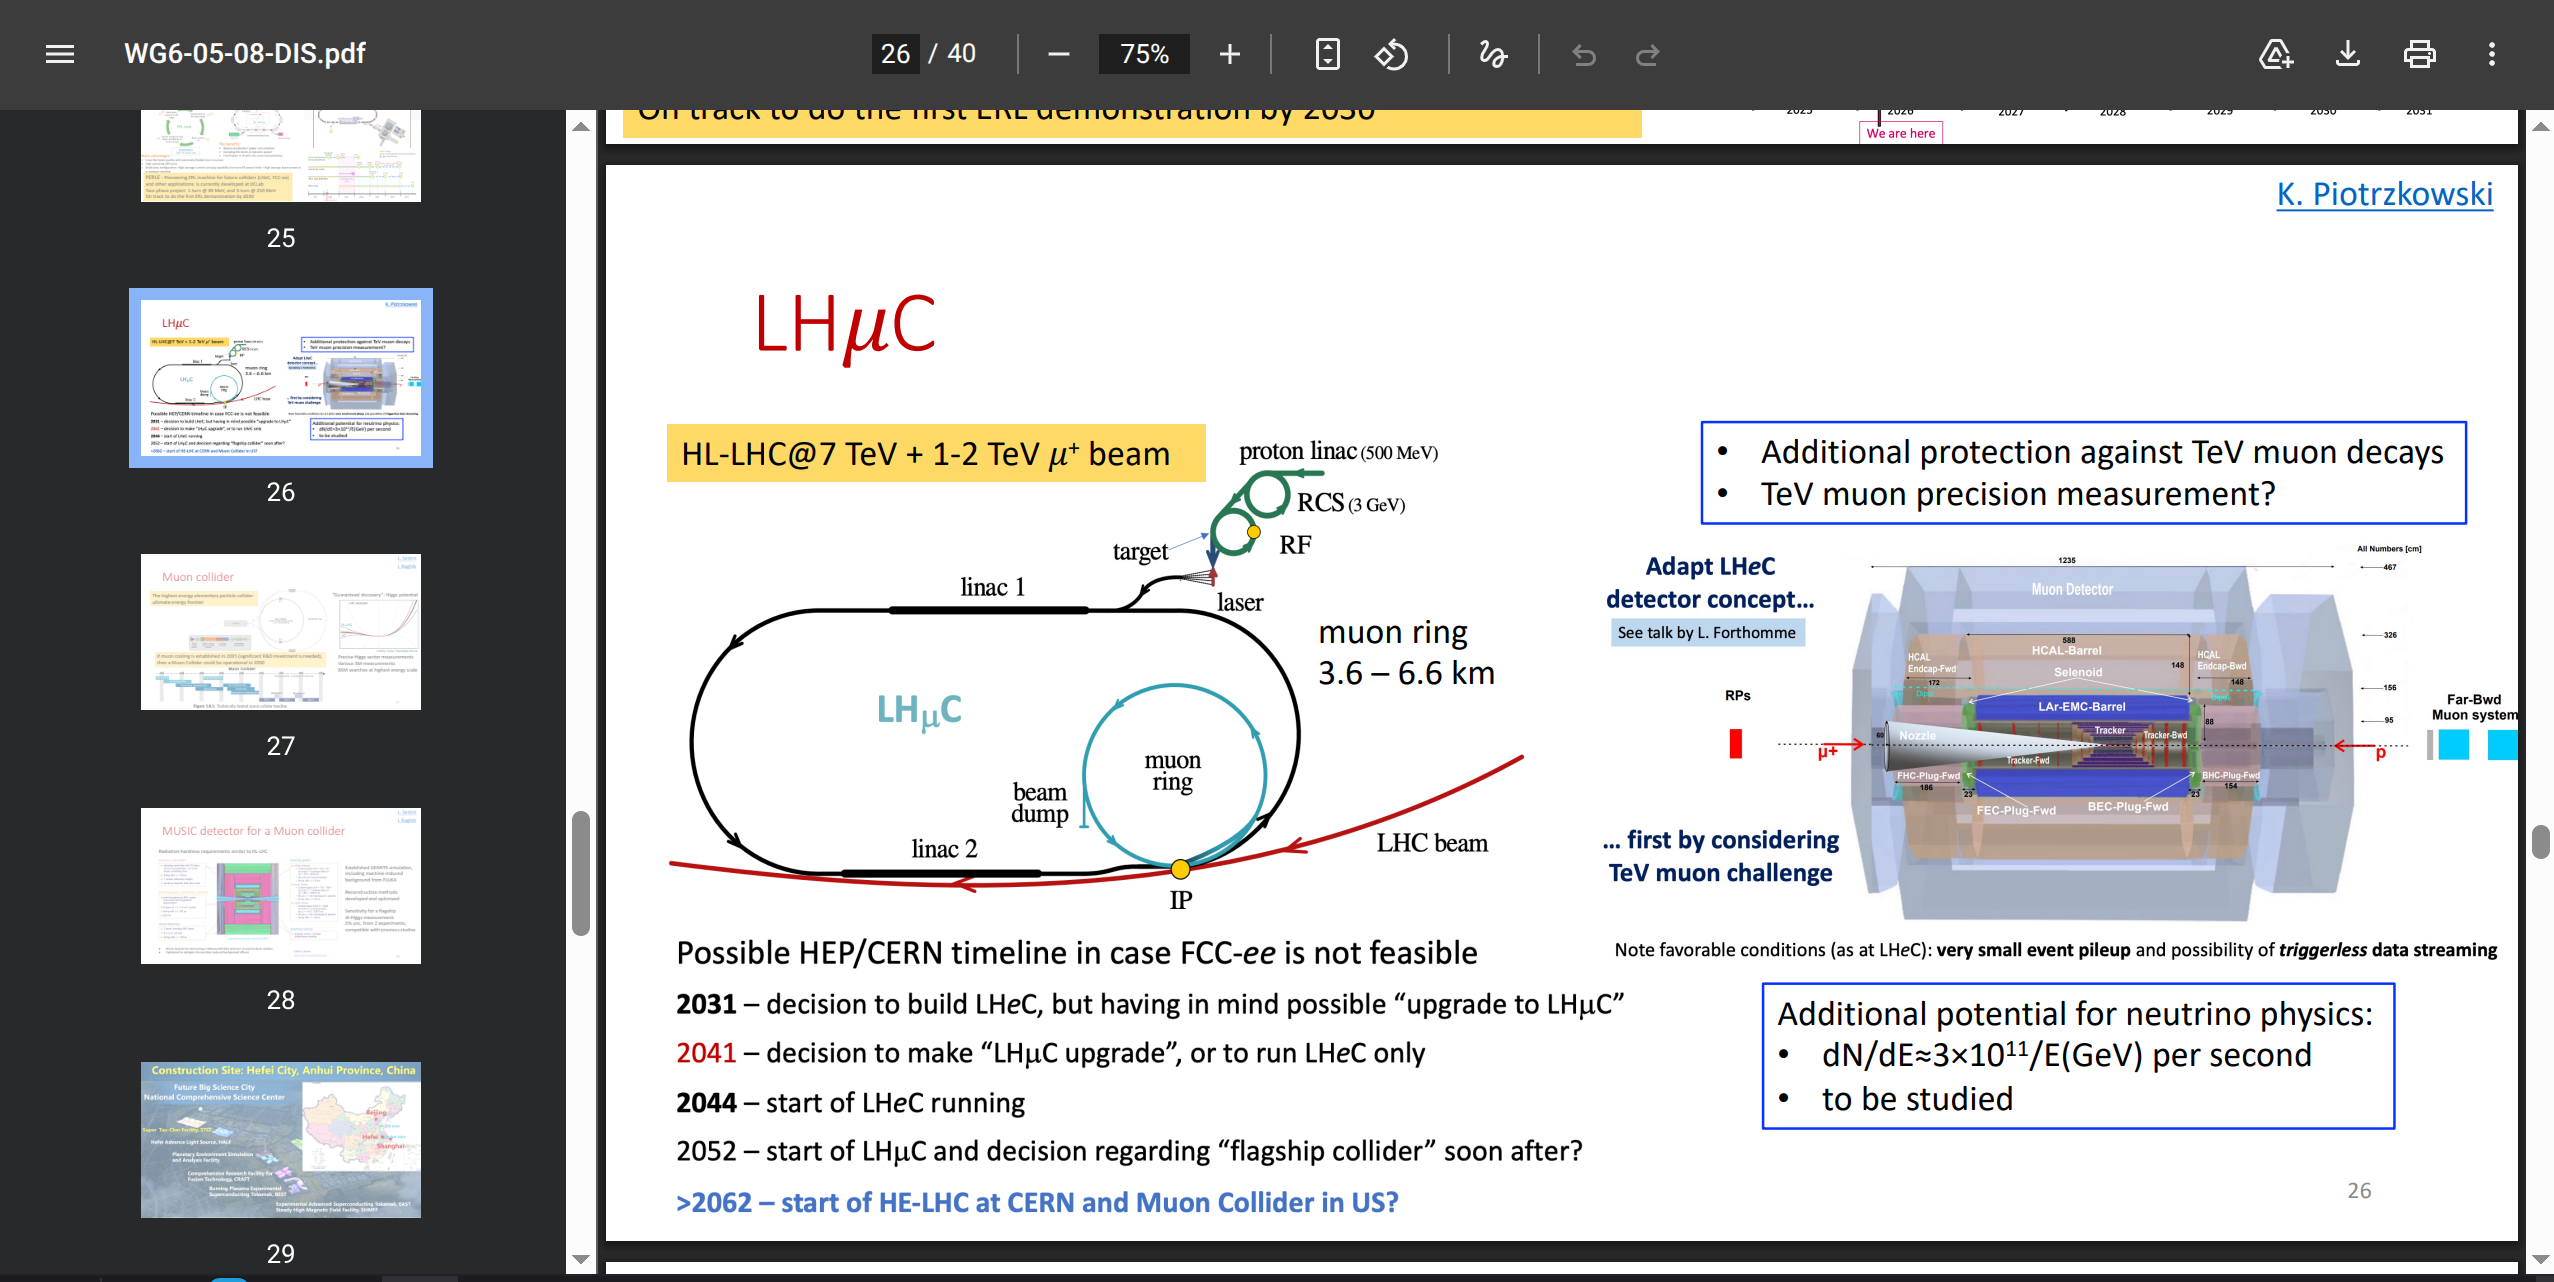
\includegraphics[width=0.85\paperwidth,height=0.85\paperheight,keepaspectratio]{Kr_1.png}
	\end{center}
	%------------------------------------------------
	% HELP4CERN logo overlay
	%------------------------------------------------
	\begin{tikzpicture}[remember picture,overlay]
		\node[anchor=north east, xshift=-0.55cm, yshift=-0.40cm]
		at (current page.north east)
		{
\includegraphics[width=1.5cm]{HELP4CERN.jpg}};
	\end{tikzpicture}
\end{frame}


% --------------------------------------------------------------------------
% Slide 11
% --------------------------------------------------------------------------



\begin{frame}{WG6 outlook: HELP4CERN white paper}
	\begin{center}
		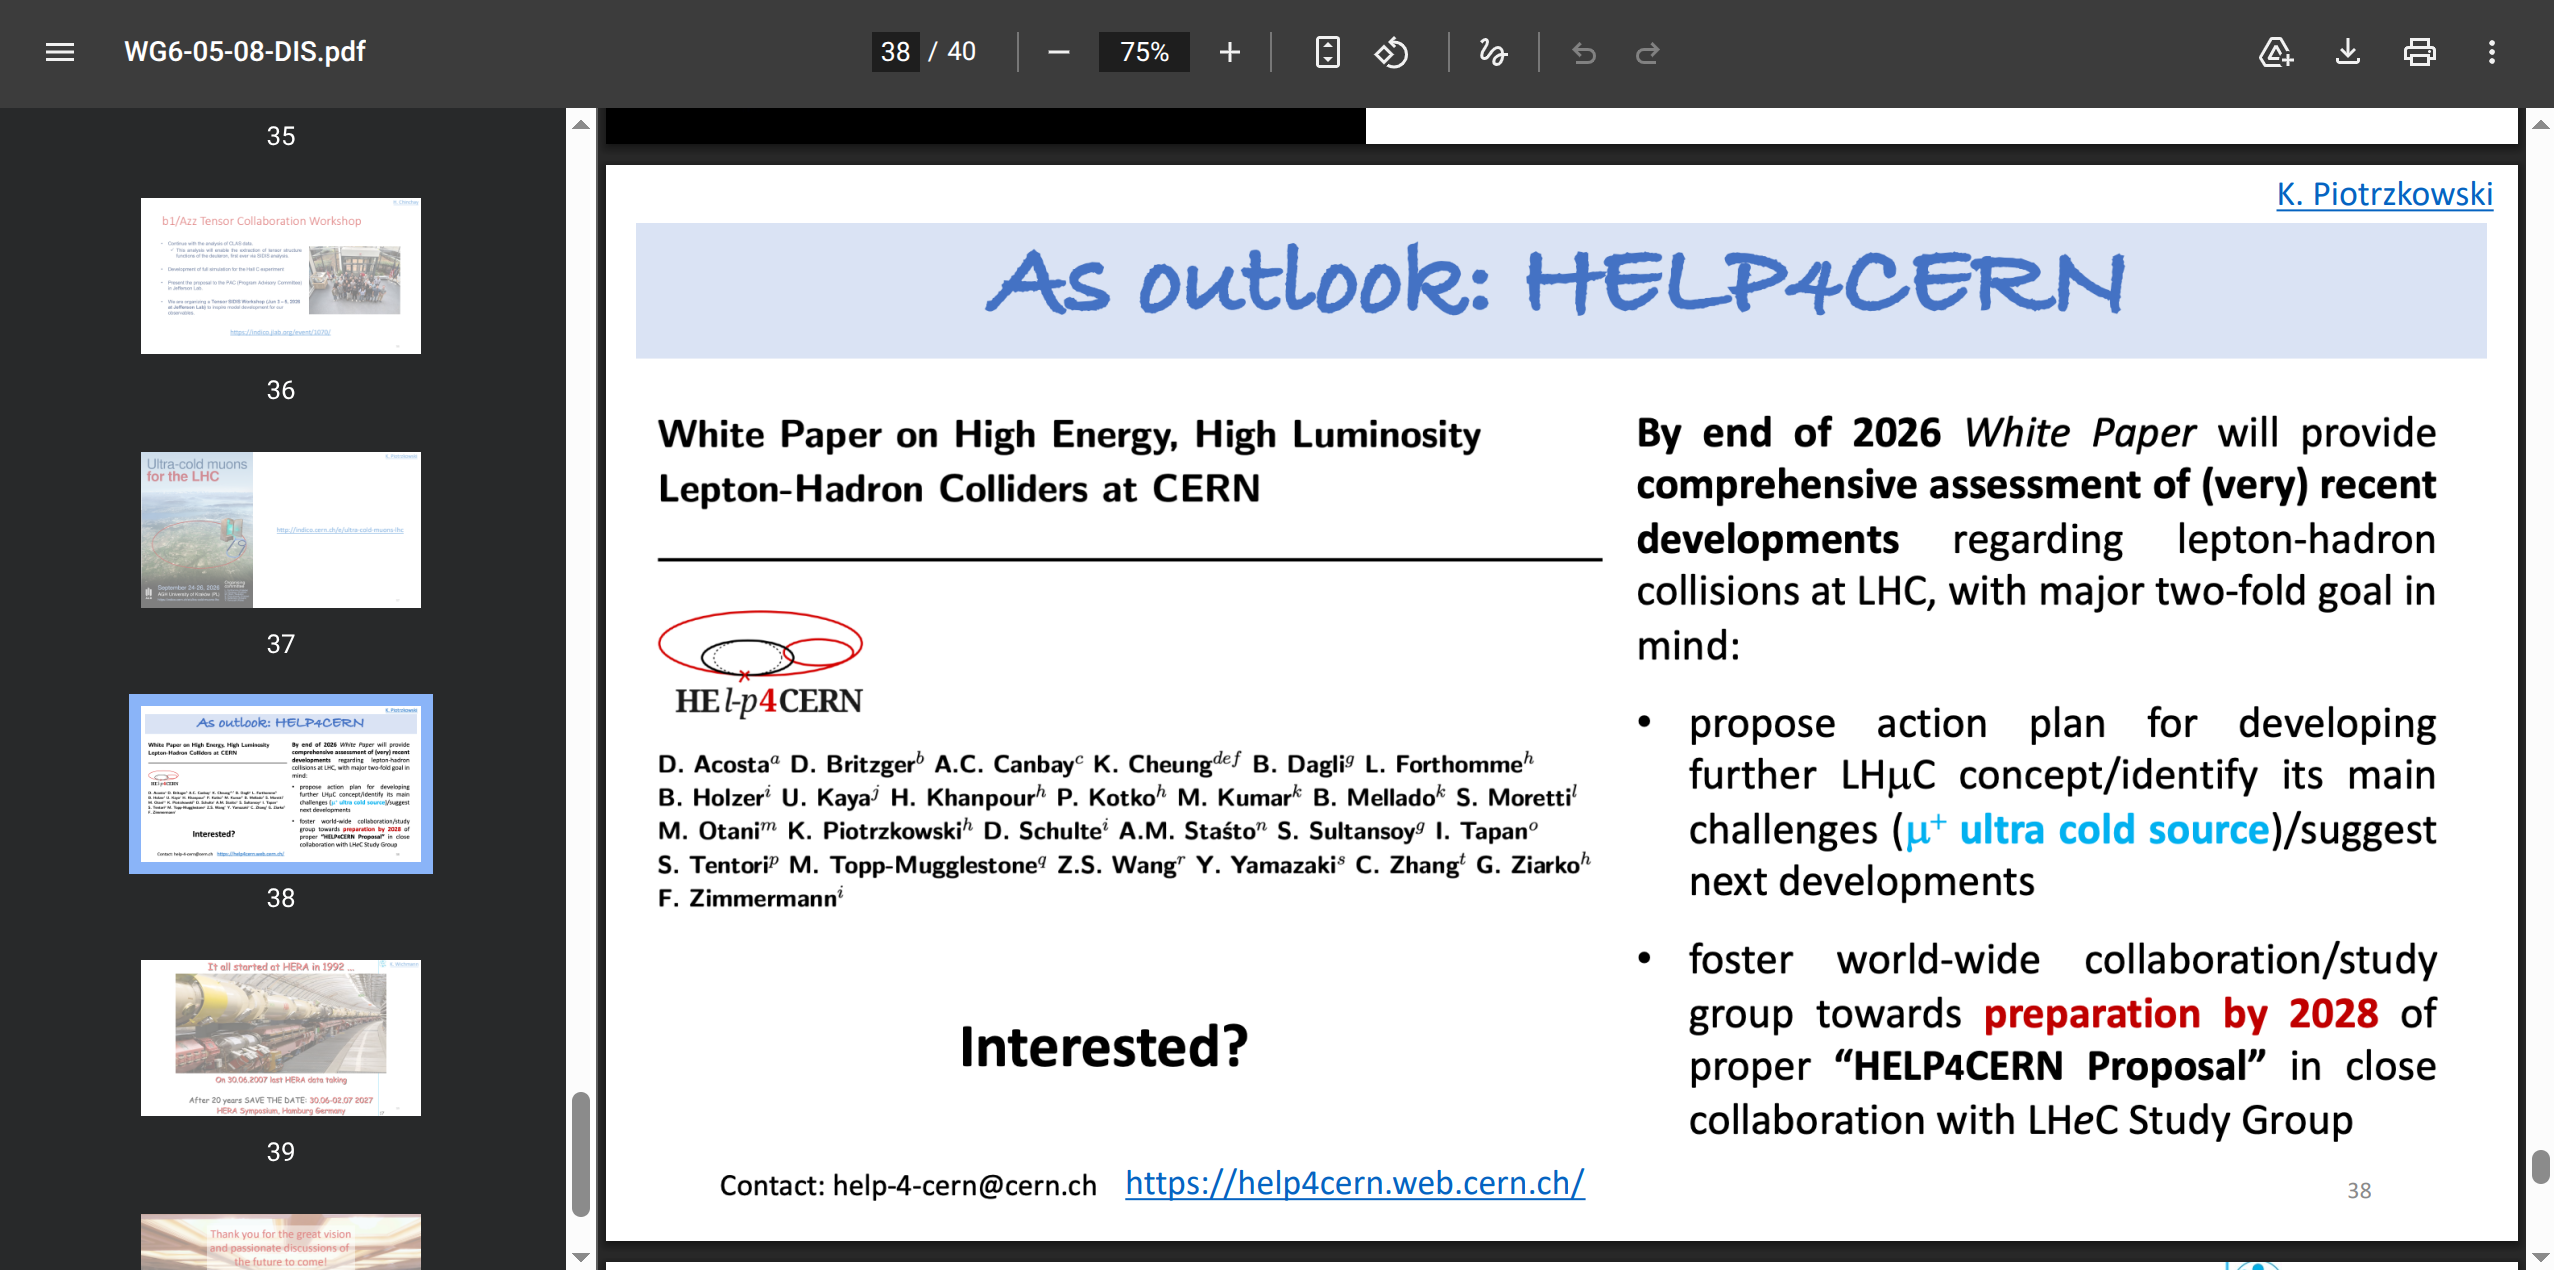
\includegraphics[width=0.85\paperwidth,height=0.85\paperheight,keepaspectratio]{Kr_2.png}
	\end{center}
	%------------------------------------------------
	% HELP4CERN logo overlay
	%------------------------------------------------
	\begin{tikzpicture}[remember picture,overlay]
		\node[anchor=north east, xshift=-0.55cm, yshift=-0.40cm]
		at (current page.north east)
		{
\includegraphics[width=1.5cm]{HELP4CERN.jpg}};
	\end{tikzpicture}
\end{frame}




% --------------------------------------------------------------------------
% Slide 12
% --------------------------------------------------------------------------


\begin{frame}{WG6 outlook: ultra-cold muons for the LHC}
	\begin{center}
		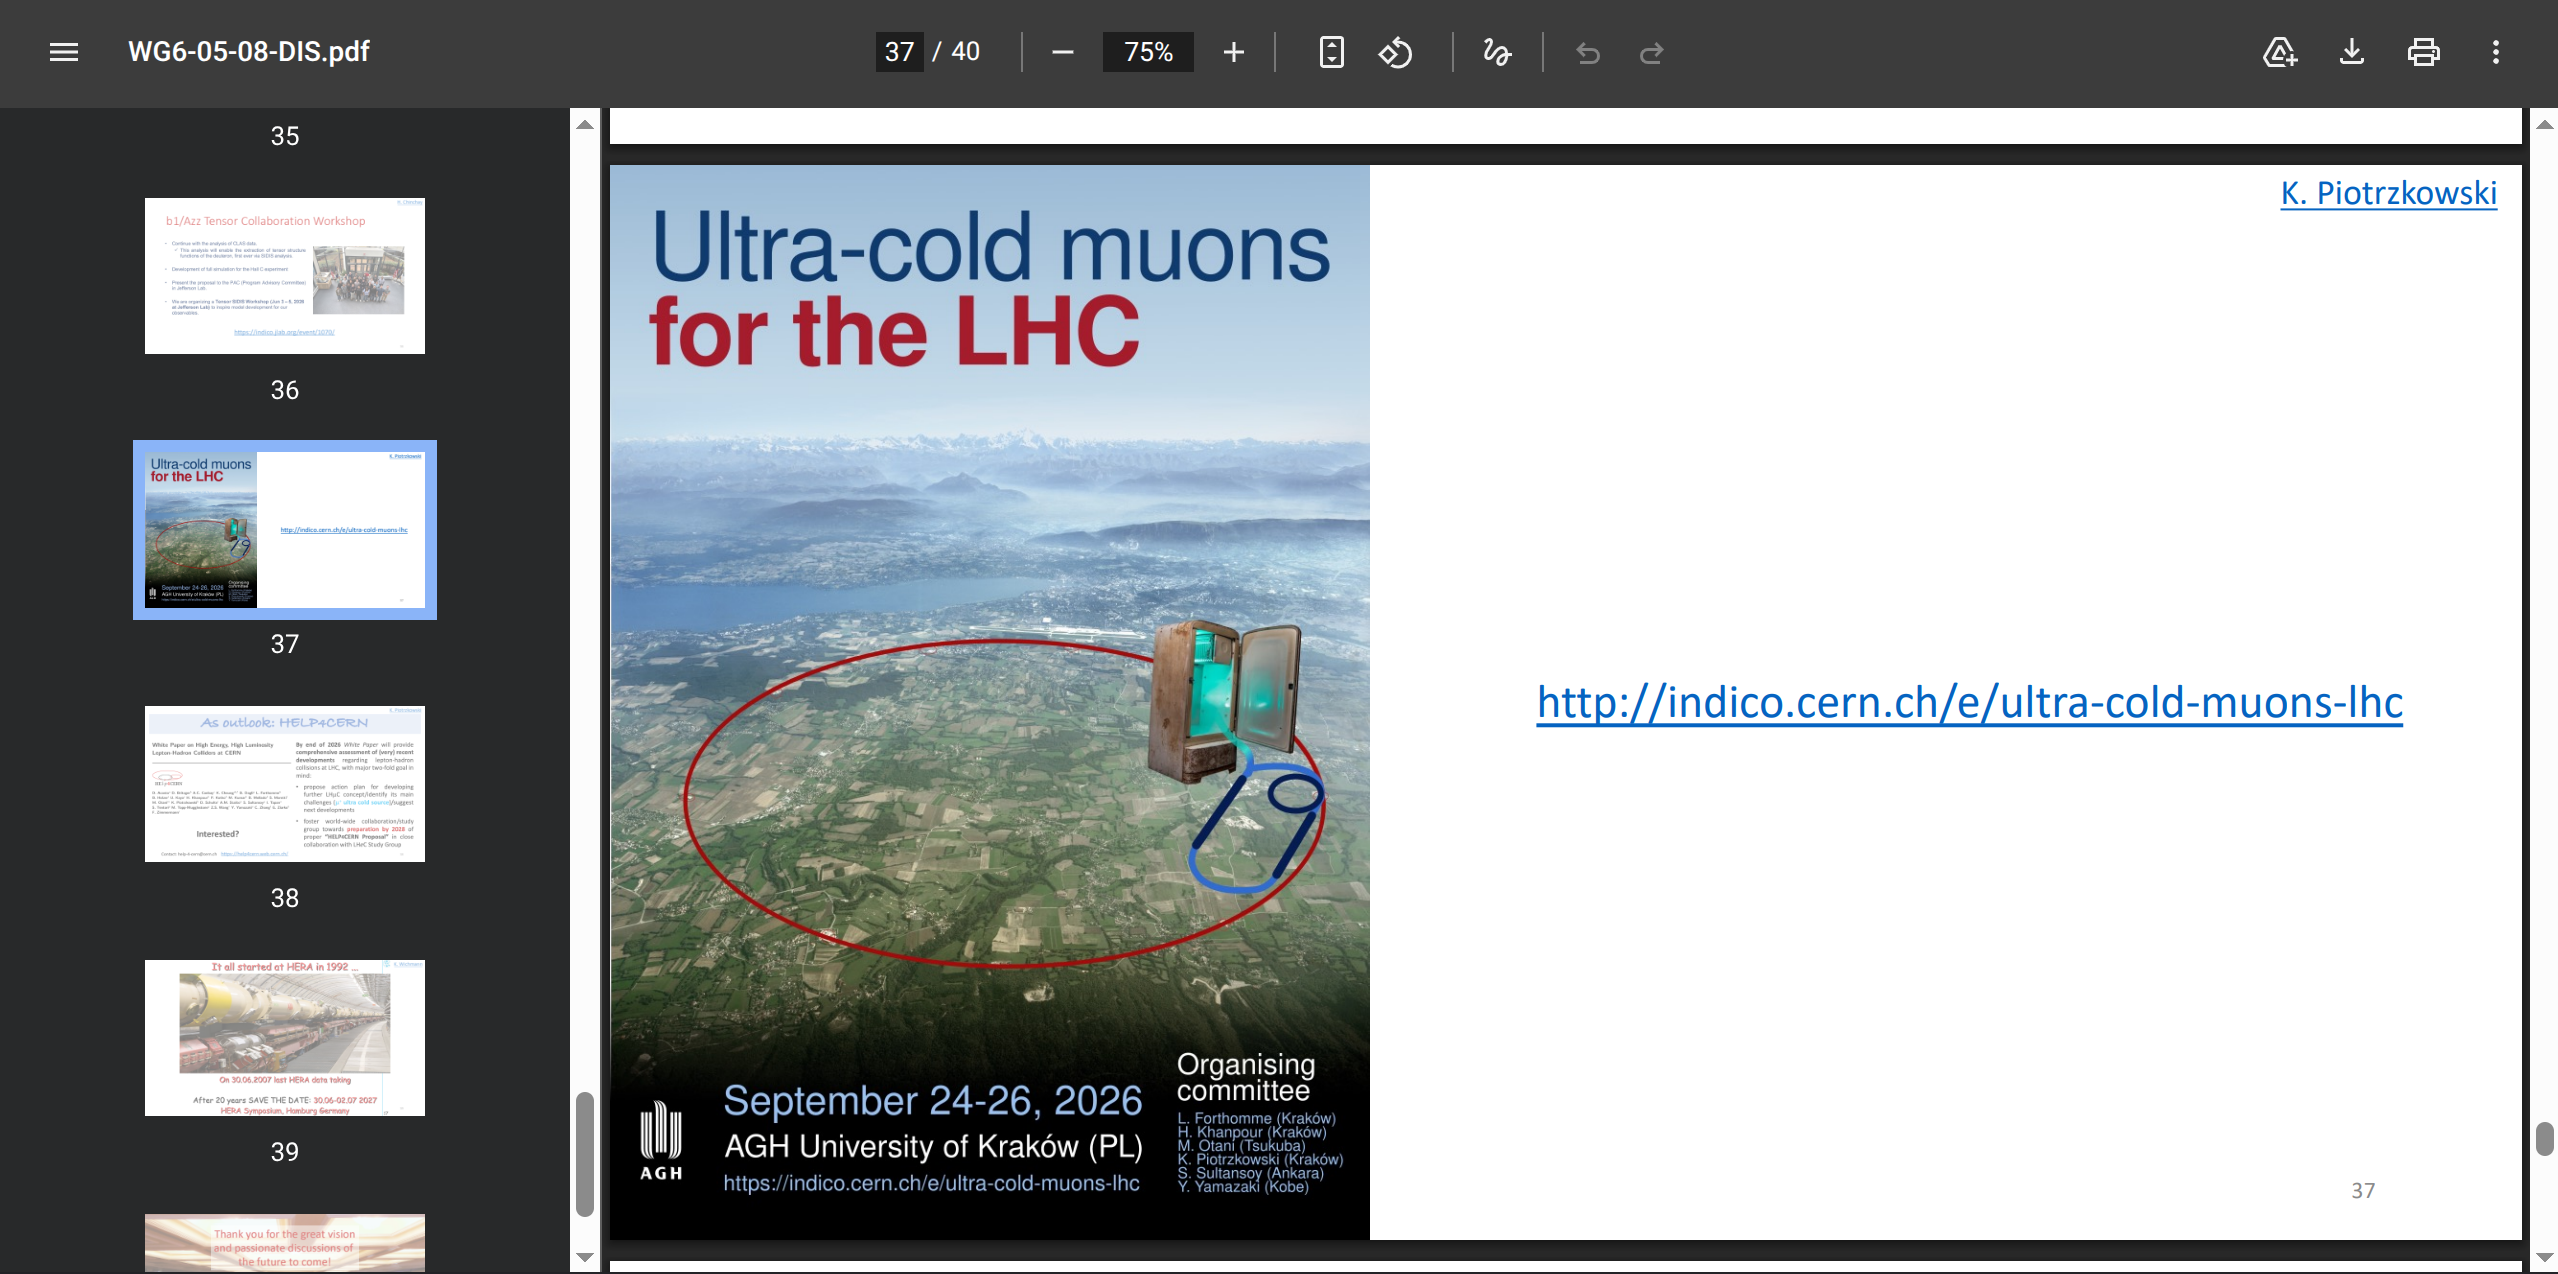
\includegraphics[width=0.85\paperwidth,height=0.85\paperheight,keepaspectratio]{Kr_3.png}
	\end{center}
	%------------------------------------------------
	% HELP4CERN logo overlay
	%------------------------------------------------
	\begin{tikzpicture}[remember picture,overlay]
		\node[anchor=north east, xshift=-0.55cm, yshift=-0.40cm]
		at (current page.north east)
		{
\includegraphics[width=1.5cm]{HELP4CERN.jpg}};
	\end{tikzpicture}
\end{frame}





% --------------------------------------------------------------------------
% Slide 13
% --------------------------------------------------------------------------


\begin{frame}{LHeC and LHeD detector concept}
	\begin{center}
		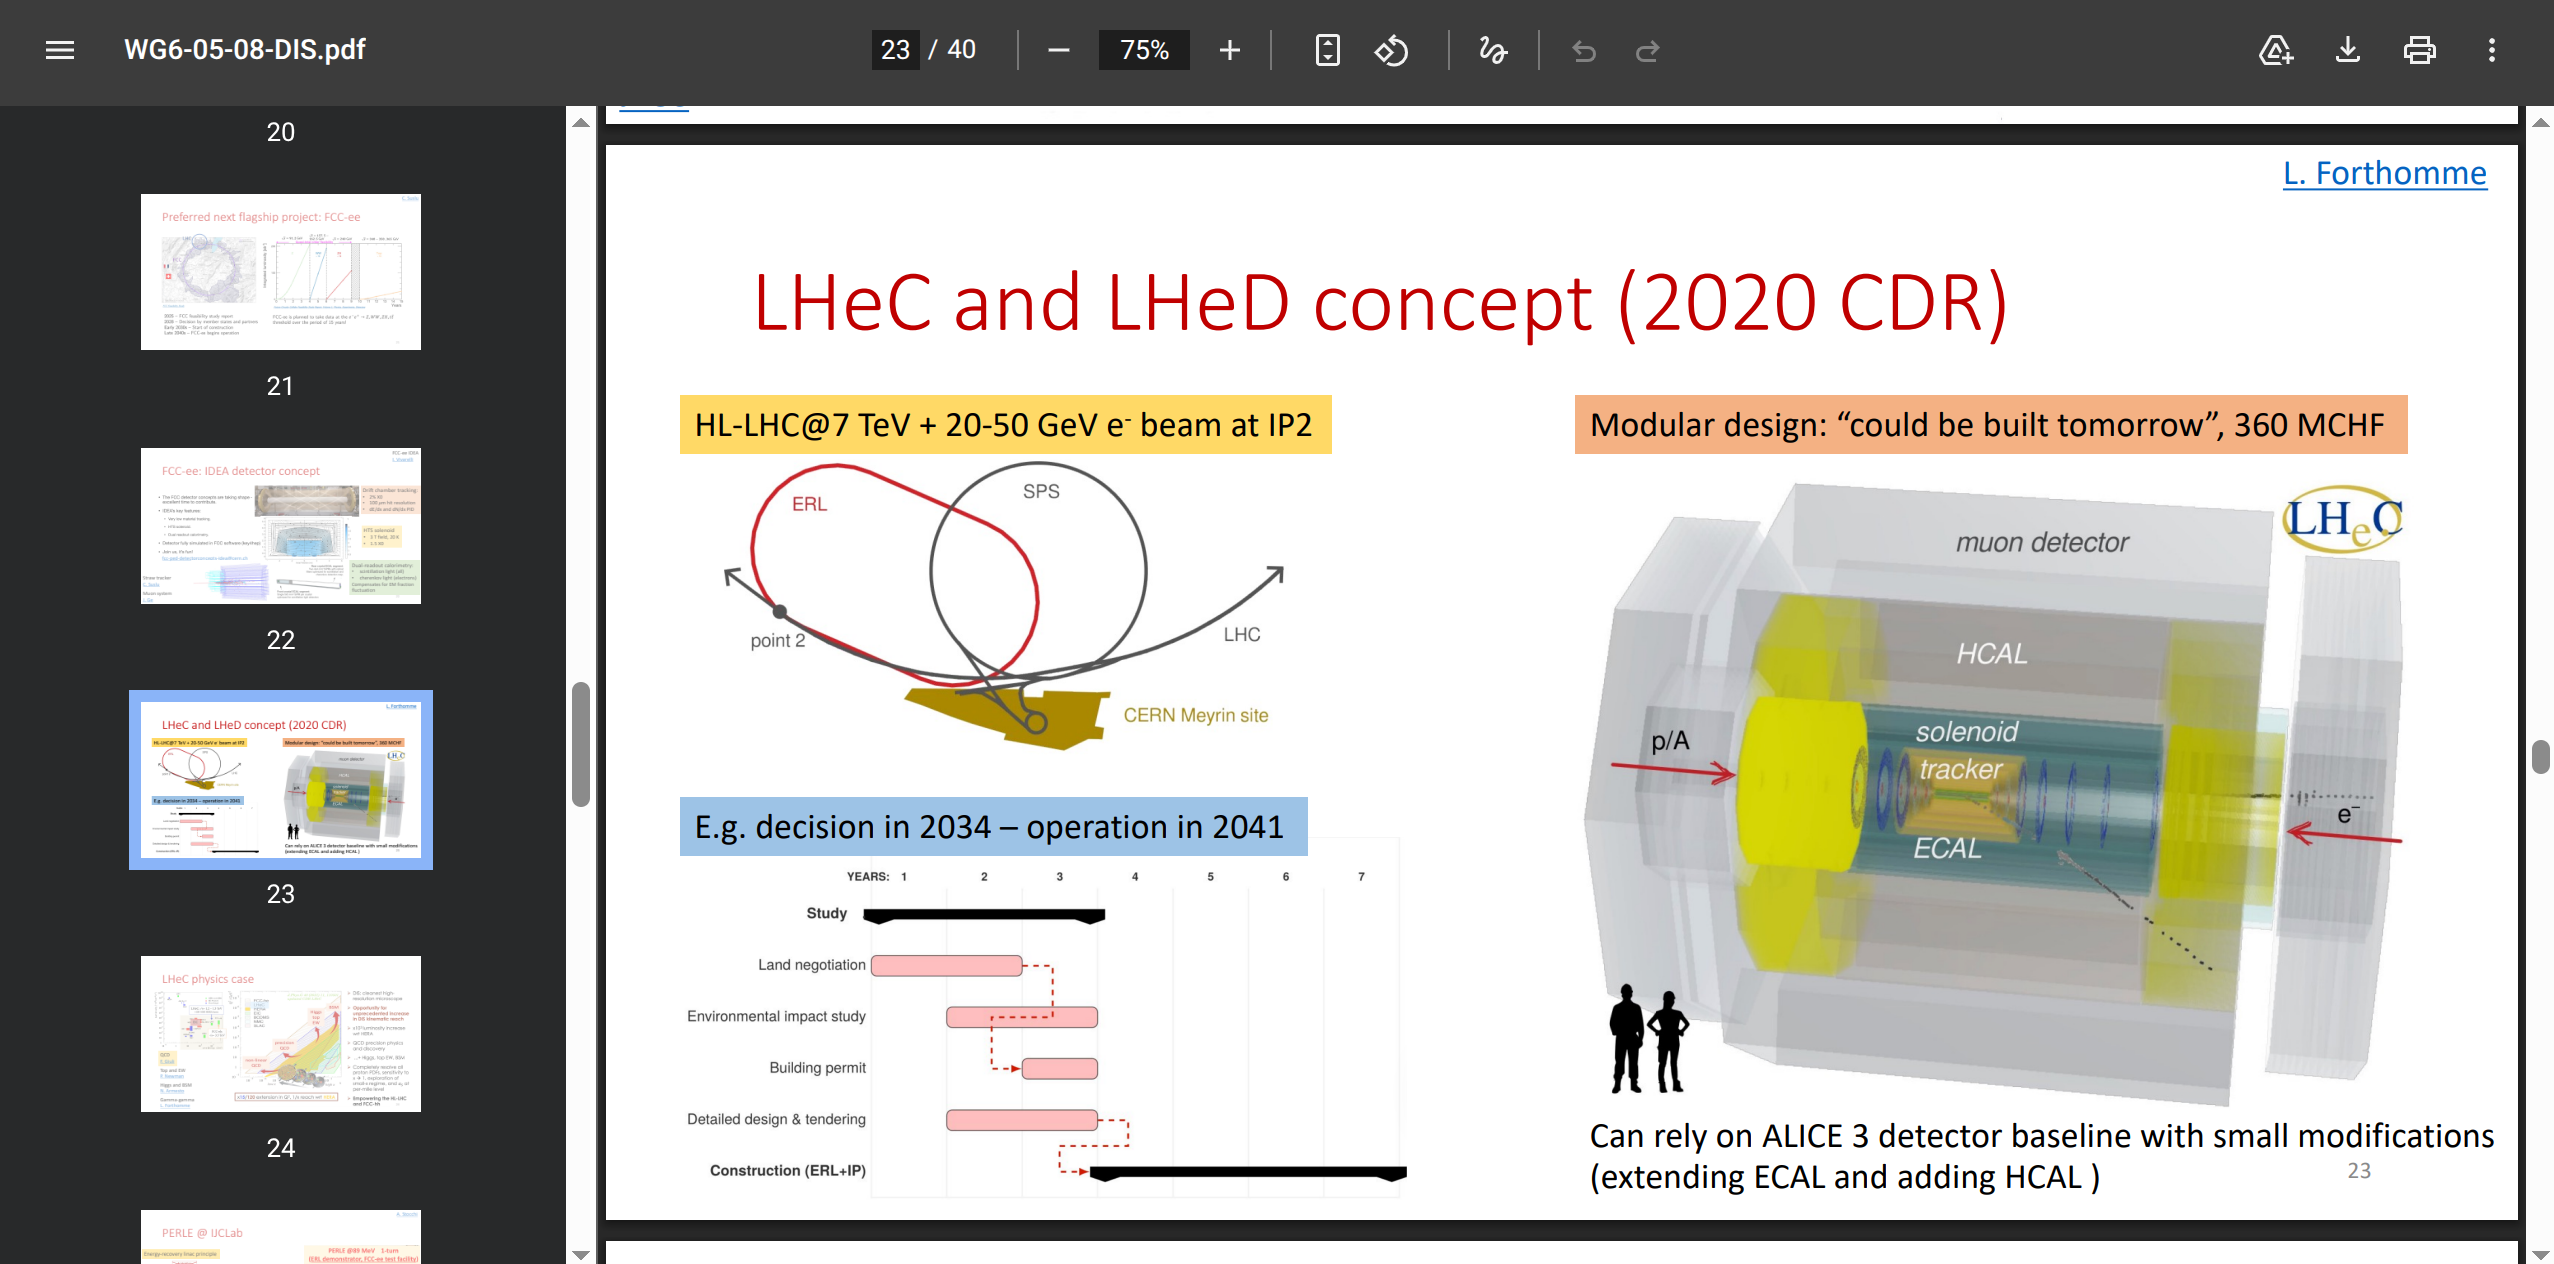
\includegraphics[width=0.85\paperwidth,height=0.85\paperheight,keepaspectratio]{La_1.png}
	\end{center}
	%------------------------------------------------
	% HELP4CERN logo overlay
	%------------------------------------------------
	\begin{tikzpicture}[remember picture,overlay]
		\node[anchor=north east, xshift=-0.55cm, yshift=-0.40cm]
		at (current page.north east)
		{
\includegraphics[width=1.5cm]{HELP4CERN.jpg}};
	\end{tikzpicture}
\end{frame}



% --------------------------------------------------------------------------
% Slide 14
% --------------------------------------------------------------------------


\begin{frame}{Staged LHeC and later LH$\mu$C extension}
	\begin{center}
		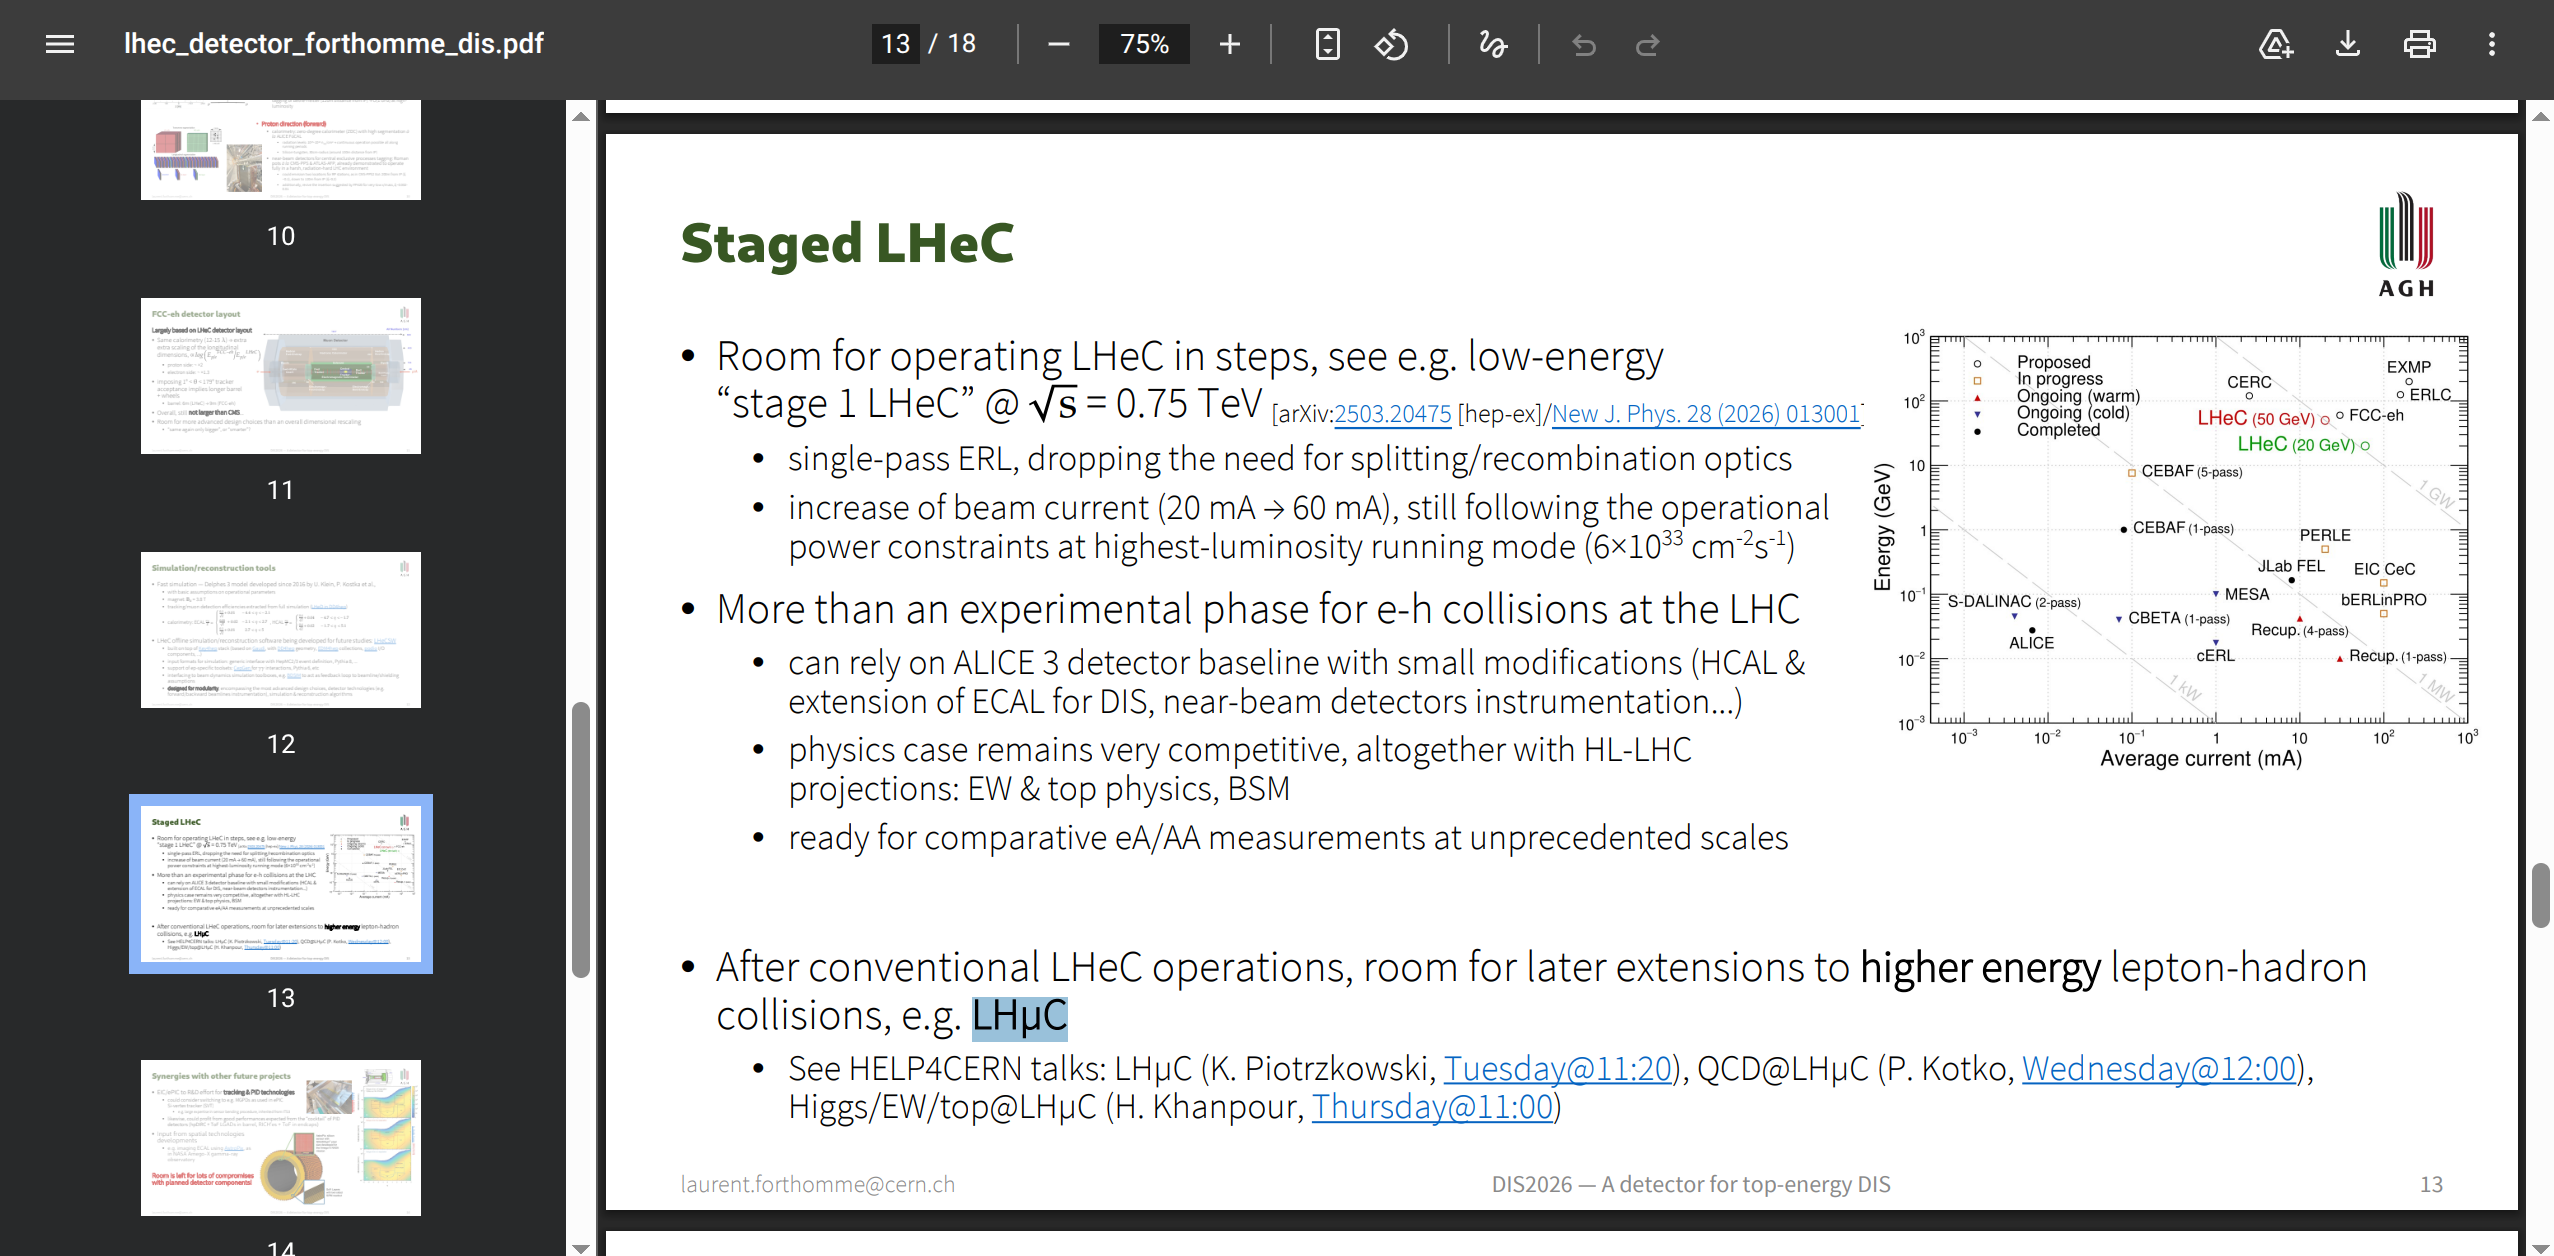
\includegraphics[width=0.85\paperwidth,height=0.85\paperheight,keepaspectratio]{La_2.png}
	\end{center}
	%------------------------------------------------
	% HELP4CERN logo overlay
	%------------------------------------------------
	\begin{tikzpicture}[remember picture,overlay]
		\node[anchor=north east, xshift=-0.55cm, yshift=-0.40cm]
		at (current page.north east)
		{
\includegraphics[width=1.5cm]{HELP4CERN.jpg}};
	\end{tikzpicture}
\end{frame}




% --------------------------------------------------------------------------
% Slide 15
% --------------------------------------------------------------------------


\begin{frame}{WG2 summary: small-$x$ physics and saturation}
	\begin{center}
		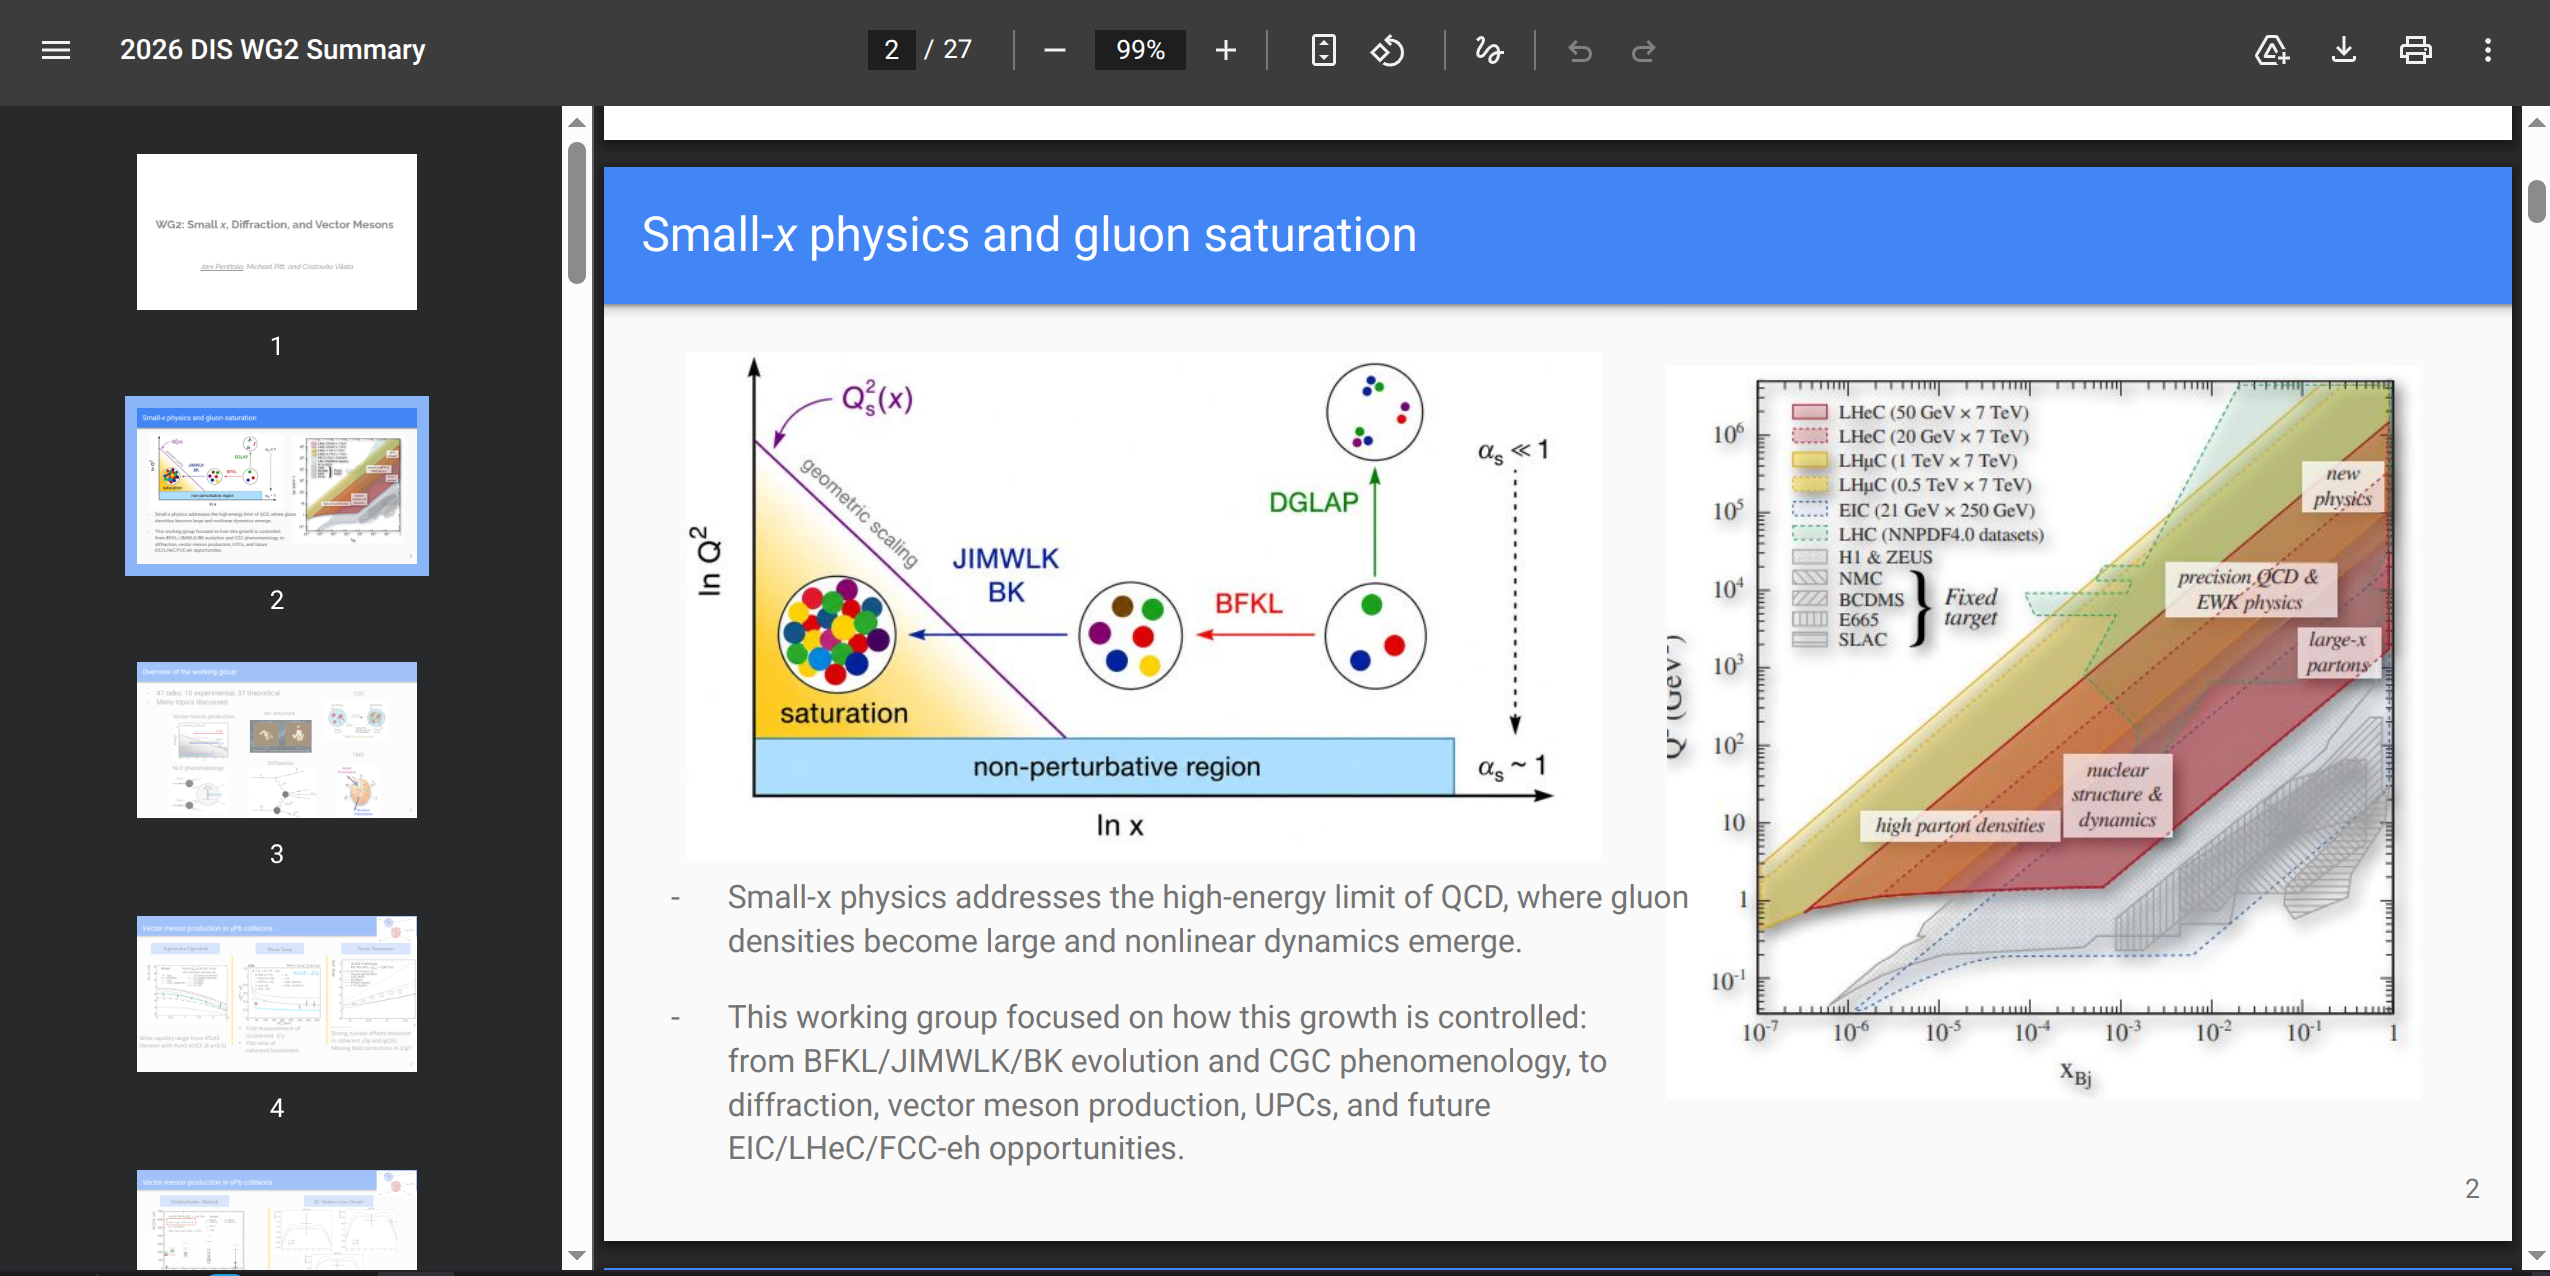
\includegraphics[width=0.85\paperwidth,height=0.85\paperheight,keepaspectratio]{Pi_1.png}
	\end{center}
	%------------------------------------------------
	% HELP4CERN logo overlay
	%------------------------------------------------
	\begin{tikzpicture}[remember picture,overlay]
		\node[anchor=north east, xshift=-0.55cm, yshift=-0.40cm]
		at (current page.north east)
		{
\includegraphics[width=1.5cm]{HELP4CERN.jpg}};
	\end{tikzpicture}
\end{frame}




% --------------------------------------------------------------------------
% Slide 16
% --------------------------------------------------------------------------


\begin{frame}{WG2 summary: new proposals for small-$x$ physics}
	\begin{center}
		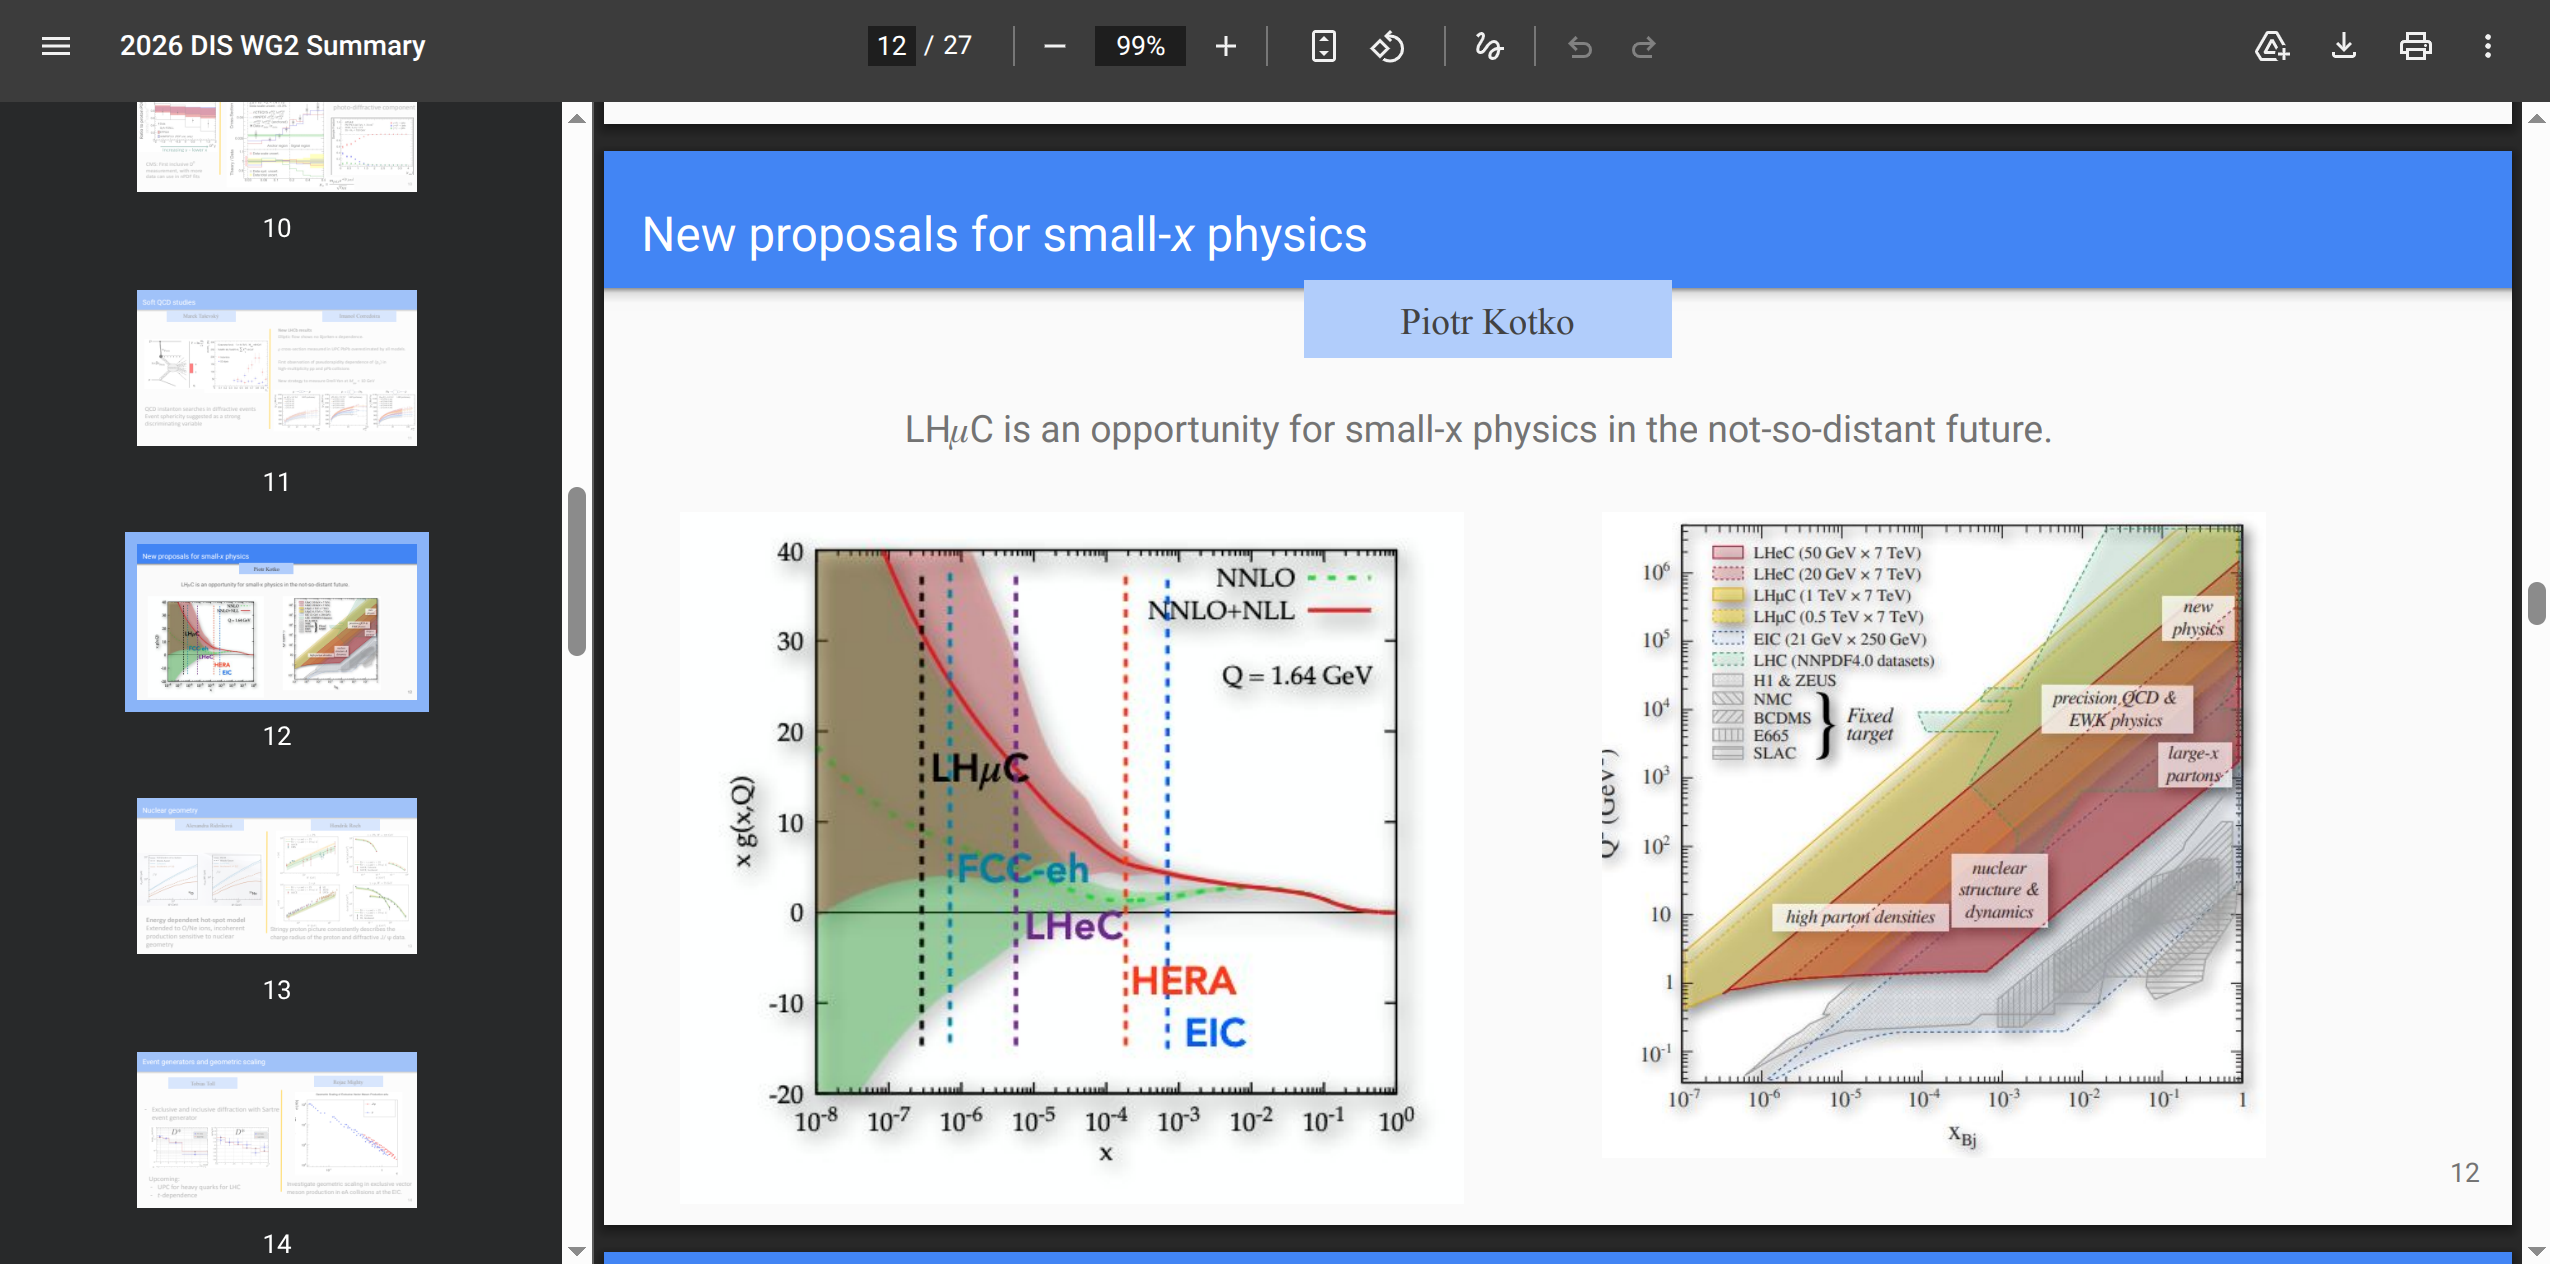
\includegraphics[width=0.85\paperwidth,height=0.85\paperheight,keepaspectratio]{Pi_2.png}
	\end{center}
	%------------------------------------------------
	% HELP4CERN logo overlay
	%------------------------------------------------
	\begin{tikzpicture}[remember picture,overlay]
		\node[anchor=north east, xshift=-0.55cm, yshift=-0.40cm]
		at (current page.north east)
		{
\includegraphics[width=1.5cm]{HELP4CERN.jpg}};
	\end{tikzpicture}
\end{frame}





\begin{frame}[plain]
\begin{center}
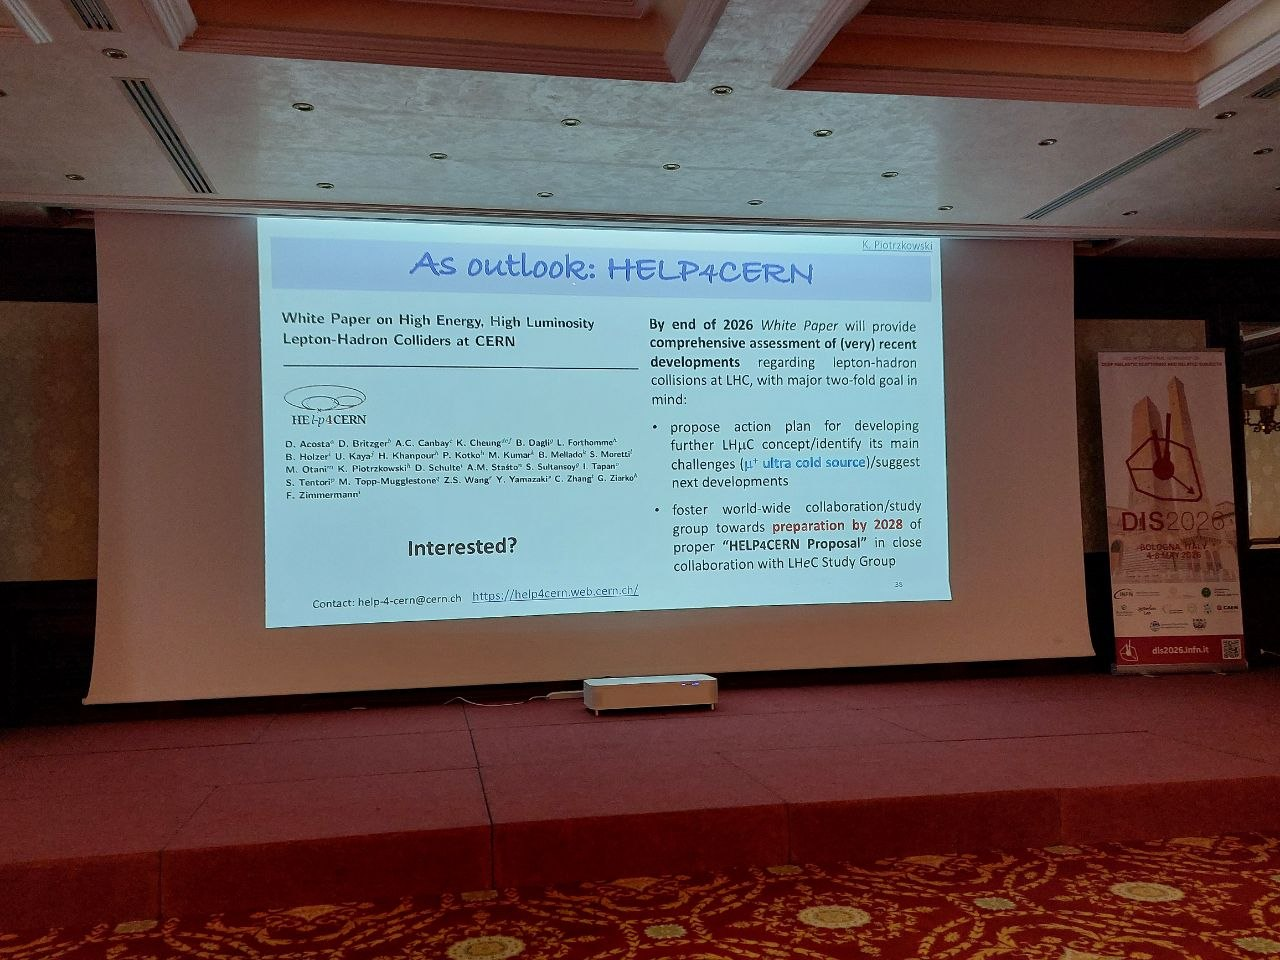
\includegraphics[width=0.85\paperwidth,height=0.85\paperheight,keepaspectratio]{1.jpg}
\end{center}
\end{frame}







\begin{frame}[plain]
	\begin{center}
		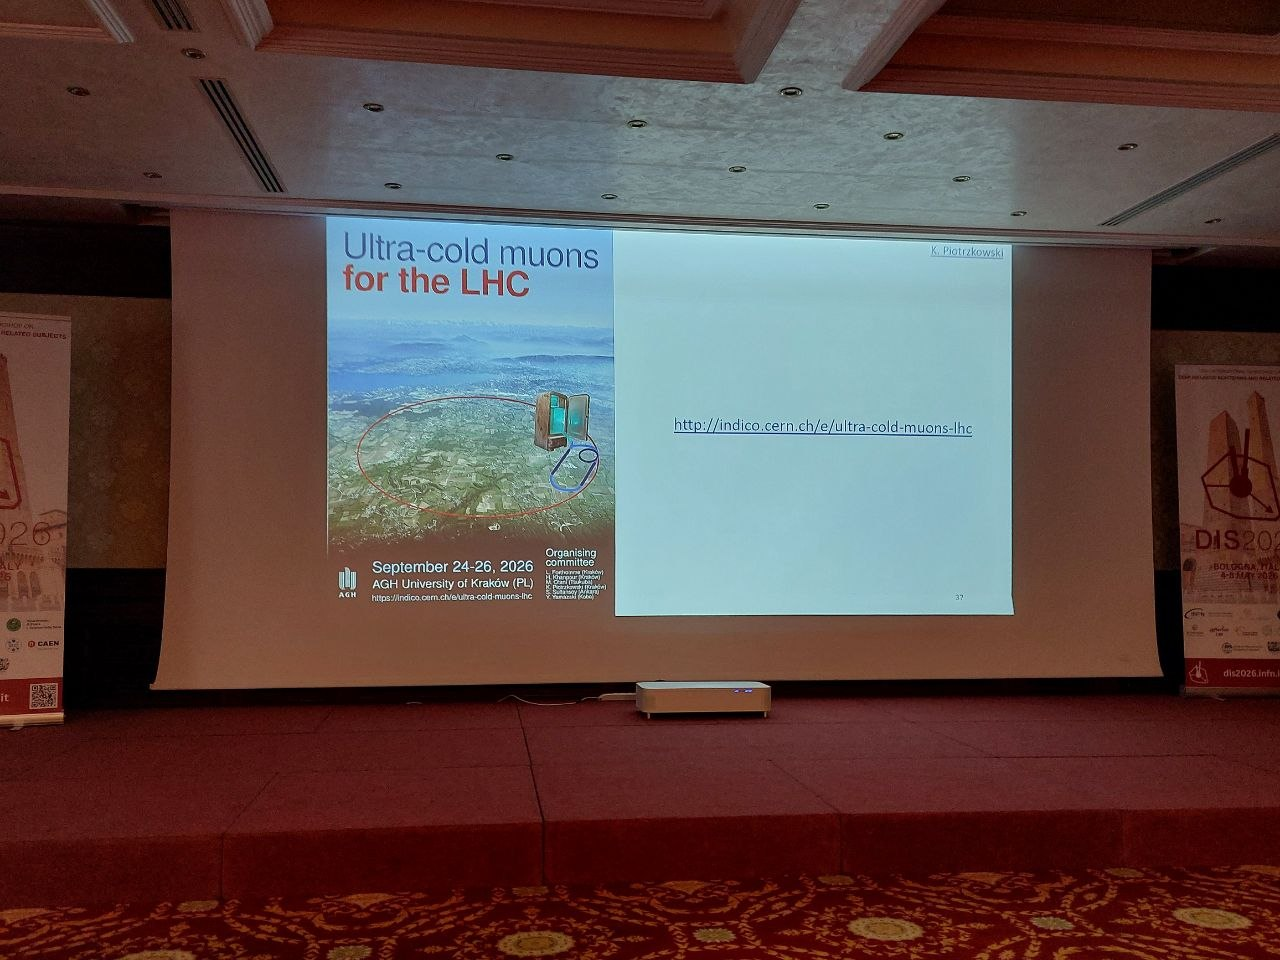
\includegraphics[width=0.85\paperwidth,height=0.85\paperheight,keepaspectratio]{2.jpg}
	\end{center}
\end{frame}







\begin{frame}[plain]
	\begin{center}
		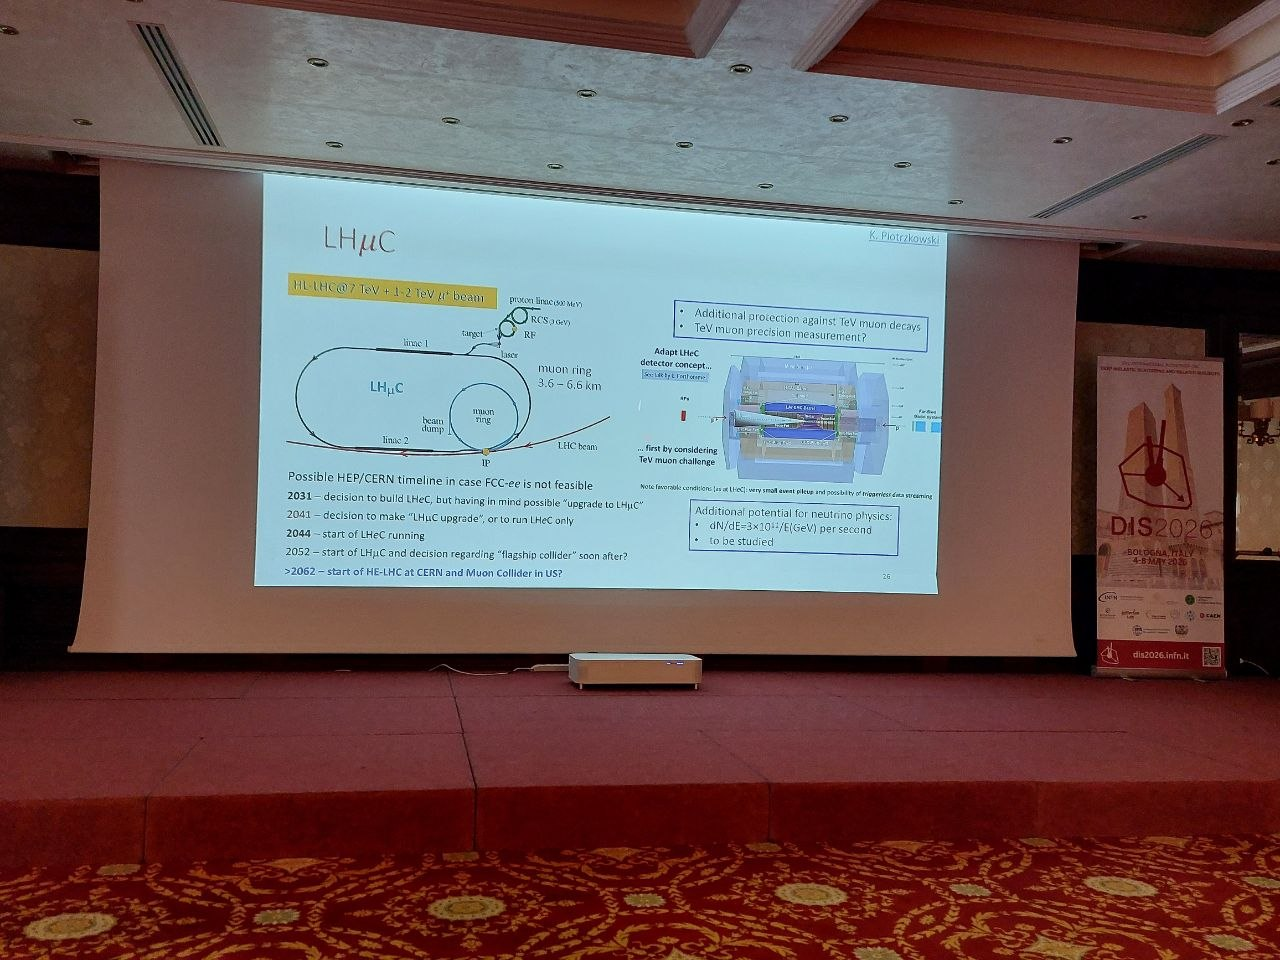
\includegraphics[width=0.85\paperwidth,height=0.85\paperheight,keepaspectratio]{3.jpg}
	\end{center}
\end{frame}







\begin{frame}[plain]
	\begin{center}
		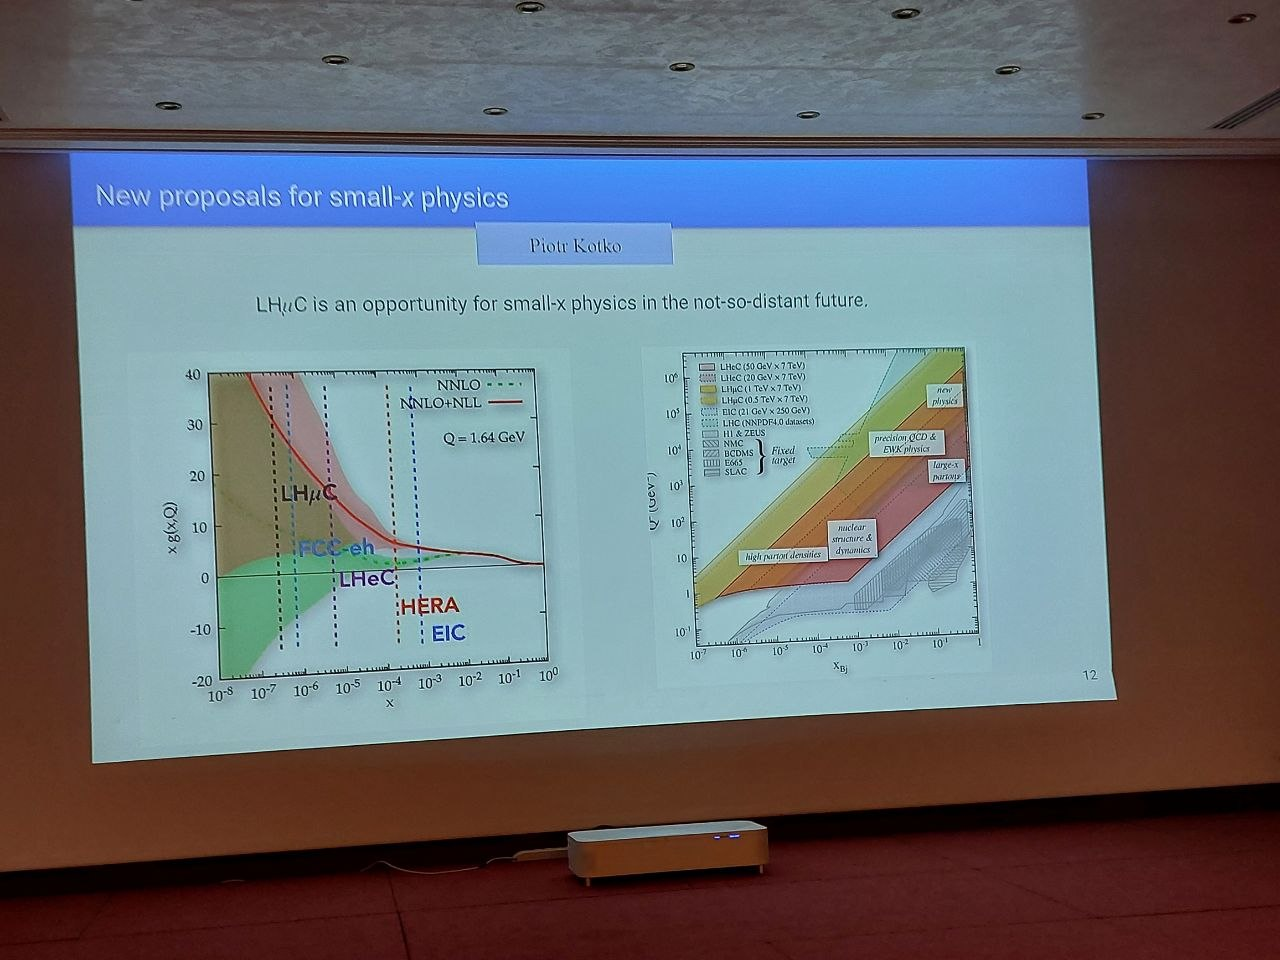
\includegraphics[width=0.85\paperwidth,height=0.85\paperheight,keepaspectratio]{4.jpg}
	\end{center}
\end{frame}
















\section{Feedback and next steps}

% --------------------------------------------------------------------------
% Slide 18
% --------------------------------------------------------------------------
\begin{frame}{DIS 2026 feedback: physics interest and next questions}
\begin{columns}[T]%[T,totalwidth=\textwidth]
\begin{column}{0.5\textwidth}
\begin{block}{What attracted attention?}
\scriptsize
\begin{itemize}
\justifying
\item The HELP4CERN proposal itself.
\item The physics potential of future lepton--hadron collisions at CERN.
\item The extended $Q^2$--$x$ plane and small-$x$ reach.
\item The complementarity with EIC, HERA and LHeC.
\end{itemize}
\end{block}
\end{column}

\begin{column}{0.5\textwidth}
\begin{exampleblock}{Physics questions to sharpen}
\scriptsize
\begin{itemize}
\justifying
\item Compare Higgs-coupling reach for HL-LHC, LHeC, LH$\mu$C and FCC-ee.
\item Emphasize complementarity: CC Higgs, high-$Q^2$ DIS, top/EW, PDFs, photon-induced channels.
\end{itemize}
\end{exampleblock}
\end{column}



\end{columns}
\reportlogonorth
\end{frame}

% --------------------------------------------------------------------------
% Slide 19
% --------------------------------------------------------------------------
\begin{frame}{From DIS 2026 to ICHEP 2026}
\begin{columns}[T]%[T,totalwidth=\textwidth]
	
\begin{column}{0.50\textwidth}
	
\begin{block}{Status after DIS 2026}
\small
\begin{itemize}
\justifying
\item The DIS talks were well received and represented in the WG summaries.
\item All four ICHEP 2026 abstracts are approved.
\item ICHEP is the next opportunity to present a coherent HELP4CERN/LHeC/LH$\mu$C programme.
\end{itemize}
\end{block}
\end{column}

\begin{column}{0.47\textwidth}
	
\begin{exampleblock}{Suggested ICHEP coordination}
\scriptsize
\begin{itemize}
\justifying
\item Use one common introductory slide across talks: concept, staging and physics pillars. 
\item Align benchmark assumptions for $\sqrt{s}$, luminosity and comparison machines. 
\item Prepare one shared slide on technical challenges. 
\end{itemize}
\end{exampleblock}
\end{column}
\end{columns}

\vspace{0.4em}
{\scriptsize
ICHEP 2026 contributions: \href{https://indico.cern.ch/event/1522800/contributions/6986580/}{6986580},
\href{https://indico.cern.ch/event/1522800/contributions/6982821/}{6982821},
\href{https://indico.cern.ch/event/1522800/contributions/6983210/}{6983210},
\href{https://indico.cern.ch/event/1522800/contributions/6980628/}{6980628}.}
\reportlogonorth
\end{frame}

% --------------------------------------------------------------------------
% Slide 21
% --------------------------------------------------------------------------
\begin{frame}[plain]
\begin{center}

\includegraphics[width=0.85\paperwidth,height=0.85\paperheight,keepaspectratio]{Thank_You_2.jpg}
\end{center}
%------------------------------------------------
% HELP4CERN logo overlay
%------------------------------------------------
\begin{tikzpicture}[remember picture,overlay]
    \node[anchor=north east, xshift=-0.55cm, yshift=-0.40cm]
    at (current page.north east)
    {
\includegraphics[width=1.5cm]{HELP4CERN.jpg}};
\end{tikzpicture}
\end{frame}




\end{document}







% --------------------------------------------------------------------------
% Slide 20
% --------------------------------------------------------------------------
\begin{frame}{Near-term actions for the HELP4CERN report}
	\begin{columns}[T]%[T,totalwidth=\textwidth]
		\begin{column}{0.48\textwidth}
			\begin{block}{Physics consolidation}
				\small
				\begin{itemize}
					\justifying
					\item Define a common benchmark table for LHeC, LH$\mu$C and long-term $\mu h$ options.
					\item Prepare consistent comparison plots for Higgs couplings and HET observables.
					\item Strengthen the QCD/small-$x$ case with clear EIC--LHeC--LH$\mu$C complementarity.
					\item Identify priority BSM benchmarks that genuinely benefit from a muon--hadron initial state.
				\end{itemize}
			\end{block}
		\end{column}
		
		\begin{column}{0.48\textwidth}
			\begin{alertblock}{Technical consolidation}
				\small
				\begin{itemize}
					\justifying
					\item Document the ultra-cold muon source assumptions and staging logic.
					\item Quantify muon-decay backgrounds and detector-protection requirements.
					\item Clarify what can be inherited from LHeC detector concepts and what is LH$\mu$C-specific.
					\item Turn DIS feedback into a focused white-paper task list.
				\end{itemize}
			\end{alertblock}
		\end{column}
	\end{columns}
	\reportlogonorth
\end{frame}



